\pdfoutput=1

\documentclass{svjour3}                     % onecolumn (standard format)
%\documentclass[smallcondensed]{svjour3}     % onecolumn (ditto)
%\documentclass[smallextended]{svjour3}       % onecolumn (second format)
%\documentclass[twocolumn]{svjour3}          % twocolumn

\smartqed  % flush right qed marks, e.g. at end of proof

\makeatletter
\renewcommand*{\@thmcounterend}{}
\makeatother
%\spnewtheorem{lemma}{Lemma}{\bfseries}{\itshape}
\spnewtheorem{assumption}{Assumption}{\bfseries}{\itshape}
%\spnewtheorem{remark}{Remark}{\bfseries}{\itshape}
\usepackage{cite}

\usepackage{slashbox} % for slashbox in tables

\usepackage{amsmath, amssymb, amsfonts}
%\newtheorem*{remark}{Remark}
%\theoremstyle{assumption}
%\newtheorem{assumption}{Assumption}
\usepackage{hyperref}
\usepackage[titletoc,toc,title]{appendix}
\usepackage{tikz}
\usepackage{hhline}
\usepackage{graphicx, color, bm}
\usepackage{subfig}
\usepackage{pgfplots}
\usepackage{pgfplotstable}
\usepackage{slopetri} % my own package for drawing triangle slopes

\renewcommand{\hat}{\widehat}
\renewcommand{\tilde}{\widetilde}

%% d in integrand
\newcommand*\diff[1]{\mathop{}\!{\mathrm{d}#1}}
\newcommand{\diag}[1]{{\rm diag}\LRp{#1}}
\newcommand{\td}[2]{\frac{{\rm d}#1}{{\rm d}{\rm #2}}}
\newcommand{\pd}[2]{\frac{\partial#1}{\partial#2}}
\newcommand{\nor}[1]{\left\| #1 \right\|}
\newcommand{\LRp}[1]{\left( #1 \right)}
\newcommand{\LRs}[1]{\left[ #1 \right]}
\newcommand{\LRa}[1]{\left\langle #1 \right\rangle}
\newcommand{\LRb}[1]{\left| #1 \right|}
\newcommand{\LRc}[1]{\left\{ #1 \right\}}
\newcommand{\LRceil}[1]{\left\lceil #1 \right\rceil}
\newcommand{\LRl}[1]{\left. #1 \right|}
\newcommand{\pdn}[3]{\frac{\partial^{#3}#1}{\partial#2^{#3}}}
\newcommand{\Grad} {\ensuremath{\nabla}}
\newcommand{\jump}[1] {\ensuremath{\llbracket#1\rrbracket}}
\newcommand{\avg}[1] {\ensuremath{\LRc{\!\{#1\}\!}}}

\renewcommand{\note}[1]{{\color{blue}{#1}}}

\graphicspath{{./figs/}}


%%%%%%%%%%%%%%%%%%%%%%%%%%%%%%%%%%%%%%%%%%%%%%%%%%%%%%%%%%%%%%%
%%%%%%%%%%%%%%%%%%%%%%%%%%%%%%%%%%%%%%%%%%%%%%%%%%%%%%%%%%%%%%%
%%%%%%%%%%%%%%%%%%%%%%%%%%%%%%%%%%%%%%%%%%%%%%%%%%%%%%%%%%%%%%%

\date{}
\author{Jesse Chan}
\title{Skew-symmetric entropy stable discontinuous Galerkin formulations}% with applications to hybrid meshes}
\titlerunning{Skew-symmetric entropy stable DG formulations}

\begin{document}

\institute{J. Chan \at 
Department of Computational and Applied Mathematics\\
Rice University\\
              6100 Main Street\\ 
              Houston, TX, 77005 \\
              \email{jesse.chan@rice.edu}
}


\maketitle

\begin{abstract}
Entropy stable high order methods for nonlinear conservation laws satisfy an inherent discrete entropy inequality.  The construction of such schemes has relied on the use of carefully chosen collocation points \cite{gassner2013skew, fisher2013high, carpenter2014entropy, crean2018entropy, chan2018efficient} or volume and surface quadrature rules \cite{chan2017discretely, chan2018discretely} to produce operators which satisfy a summation-by-parts (SBP) property.  In this work, we show how to construct skew-symmetric schemes which are entropy stable even for volume and surface quadratures under which a traditional SBP property does not hold.  These skew-symmetric formulations avoid the use of a ``strong'' SBP property, and require only that operators exactly differentiate constants and satisfy a discrete form of the fundamental theorem of calculus.   We conclude with an application of the skew-symmetric formulation for entropy stable schemes on mixed quadrilateral-triangle meshes. 
\end{abstract}

%\tableofcontents

\section{Introduction}

High order methods for the simulation of time-dependent compressible flow have the potential to achieve higher levels of accuracy at lower costs compared to current low order schemes \cite{wang2013high}.  In addition to superior accuracy, the low numerical dispersion and dissipation of high order methods \cite{ainsworth2004dispersive} enables the accurate propagation of waves over long distances and time scales.  The same properties also make high order methods attractive for unsteady phenomena such as vorticular and turbulent flows, which are sensitive to numerical dissipation \cite{visbal1999high, wang2013high}.  

However, when applied to nonlinear conservation laws, high order methods can experience artificial growth and blow-up near under-resolved features such as shocks, turbulence, or boundary layers.  In practice, the application of high order methods to practical problems requires shock capturing and stabilization techniques (such as artificial viscosity) or solution regularization (such as filtering or limiting) to prevent solution blow-up.  The resulting schemes for nonlinear conservation laws walk a fine line between stability, robustness, and accuracy.  Aggressive stabilization or regularization can result in the loss of high order accuracy, while too little can result in instability \cite{wang2013high}.  Moreover, it can be difficult to determine robust expressions for stabilization paramaters, as parameters which work for one simulation can fail when applied to a different physical regime or discretization setting.  

These issues have motivated the introduction of high order \textit{entropy stable} discretizations, which satisfy a semi-discrete entropy inequality while maintaining high order accuracy in smooth regions.  Proofs of continuous entropy inequalities rely on the chain rule, which does not hold discretely due to effects such as quadrature error.   By using an approach referred to as ``flux differencing'', entropy stable schemes account for the loss of the chain rule while maintaining a semi-discrete analogue of the continuous entropy inequality.  These schemes were first introduced as high order collocation methods on tensor product elements in \cite{fisher2013high, carpenter2014entropy, gassner2016split, gassner2017br1}, and were extended to simplicial elements in \cite{crean2017high, chen2017entropy, crean2018entropy, chan2017discretely, chan2018discretely}.  Entropy stable methods have also been extended to a variety of other discretization settings, including staggered grids \cite{parsani2016entropy}, Gauss-Legendre collocation \cite{chan2018efficient}, and non-conforming meshes \cite{friedrich2017entropy}.  

Entropy stable discretizations are built upon flux differencing and a summation-by-parts (SBP) property, which serves as a discrete analogue of integration by parts for quadrature-based discretization matrices.  However, the SBP property does not hold for some under-integrated quadrature rules, which naturally arise in certain discretization settings.  For example, on hybrid meshes consisting of both quadrilateral and triangular elements, it is convenient to utilize the same quadrature rule on shared faces between different element types.  On degree $N$ tensor product elements, a popular choice of quadrature is an $(N+1)$-point Gauss-Legendre-Lobatto (GLL) rule.  When both volume and surface integrals are approximated using $(N+1)$ point GLL quadrature rules, the SBP property holds, despite the fact that GLL quadrature is inexact for the integrands which appear in finite element formulations \cite{fisher2013high}.  However, while GLL quadrature induces an SBP property on quadrilateral elements, but does not always result in an SBP property if used for triangular elements \cite{chan2017discretely}.  %A similar issue arises on non-conforming meshes, where a composite ``split-side'' quadrature naturally when coupling larger elements to smaller elements through a non-conforming interface \cite{kozdon2018energy}.  For quadrilaterals utilizing a GLL volume quadrature, the use of a composite quadrature on a non-conforming face also results in the loss of the SBP property \cite{chan2017discretely}.  

This work proposes an alternative formulation which utilizes a skew-symmetric form of flux differencing.  Under such a formulation, the proof of entropy stability requires only a weaker ``variational'' form of the SBP property, which holds under a more general class of quadrature rules compared to the decoupled SBP property introduced in \cite{chan2017discretely, chan2018discretely}.  We show that the skew-symmetric formulation is entropy stable, locally conservative, and free-stream preserving on curved elements, and confirm theoretical results with numerical experiments on triangular, quadrilateral, and hybrid triangular-quadrilateral meshes.  

It should be noted that a similar approach to entropy stable discretizations was introduced within a finite difference framework \cite{chen2017entropy, crean2018entropy} using multidimensional differencing operators which are constructed to satisfy accuracy conditions and an SBP property \cite{hicken2016multidimensional}.  These operators do not correspond to any specific basis or approximation space, but can be shown to exist for nodal points corresponding to sufficiently accurate choices of volume and surface quadrature and can be computed either algebraically or through an optimization problem.  The formulations presented in this work require similar accuracy conditions, but differ from those of \cite{chen2017entropy, crean2018entropy} in that we start with an explicit approximation space, which then induce quadrature-based operators.  The formulations presented here also accomodate general choices of volume and surface quadrature (e.g.\ volume quadratures without boundary nodes and over-integrated rules) while ensuring compact coupling conditions between neighboring elements.  

The structure of the paper is as follows: Section~\ref{sec:nonlin} describes the continuous entropy inequality which we aim to replicate discretely.  Section~\ref{sec:approx} and Section~\ref{sec:sbp} introduce polynomial approximation spaces and quadrature-based SBP operators on simplicial and tensor product elements.  Section~\ref{sec:skew1} then introduces the variational SBP property and an entropy conservative skew-symmetric formulation.  Section~\ref{sec:skew2} extends the skew-symmetric formulation to curved elements, and Section~\ref{sec:num} presents numerical experiments which verify the theoretical assumptions, stability, and accuracy of the proposed formulations.

%\note{Finish: add Section description.  Talk about situations where the SBP or decoupled SBP property doesn't hold: triangles with reduced surface quadrature, GLL quads with GQ face quadratures, and hybrid couplings.}


\section{Entropy stability for systems of nonlinear conservation laws}
\label{sec:nonlin} 

We begin by reviewing the dissipation of entropy for a $d$-dimensional system of nonlinear conservation laws on a domain $\Omega$
\begin{equation}
\pd{\bm{u}_h}{t}  + \sum_{j=1}^d\pd{\bm{f}_j(\bm{u})}{x_j} = 0, \qquad \bm{u}\in \mathbb{R}^n, \qquad \bm{f}:\mathbb{R}^n\rightarrow\mathbb{R}^n,
\label{eq:nonlineqs}
\end{equation}
where $\bm{u}$ are the conservative variables and $\bm{f}(\bm{u})$ is a vector-valued nonlinear flux function.  We are interested in nonlinear conservation laws for which a convex entropy function $U(\bm{u})$ exists.  For such systems, the  \emph{entropy variables} are an invertible mapping $\bm{v}(\bm{u}):\mathbb{R}^n\rightarrow \mathbb{R}^n$ defined as the derivative of the entropy function with respect to the conservative variables 
\begin{align}
\bm{v}(\bm{u}) = \pd{U}{\bm{u}}.%, \qquad  \text{ invertible}.%\bm{u}\LRp{\bm{v}(\bm{u})} = \bm{u}.
\label{eq:entropyvarsmap}
\end{align}
Several widely used equations in fluid modeling (Burgers, shallow water, compressible Euler and Navier-Stokes equations) yield convex entropy functions $U(\bm{u})$ \cite{hughes1986new, chen2017entropy}.  Let $\partial \Omega$ be the boundary of $\Omega$ with outward unit normal $\bm{n}$.  By multiplying the equation (\ref{eq:nonlineqs}) with $\bm{v}(\bm{u})^T$, the solutions $\bm{u}$ of (\ref{eq:nonlineqs}) can be shown to satisfy an entropy inequality
\begin{equation}
\int_{\Omega}\pd{U(\bm{u})}{t}\diff{x} + \int_{\partial \Omega} \sum_{j=1}^d \LRp{\bm{v}(\bm{u})^T\bm{f}_j(\bm{u}) - \psi_j\LRp{\bm{v}(\bm{u})}}n_j \diff{x} \leq 0, 
\label{eq:entropyineq}
\end{equation}
where $\bm{n} = \LRp{n_1,\ldots,n_d}$ denotes the outward unit normal, and $\psi_j(\bm{u})$ is some function referred to as the entropy potential.  

The proof of (\ref{eq:entropyineq}) requires the use of the chain rule \cite{mock1980systems, harten1983symmetric, dafermos2005compensated}.  The instability-in-practice of high order schemes for (\ref{eq:nonlineqs}) can be attributed in part to the fact that the discrete form of the equations do not satisfy the chain rule, and thus do not satisfy (\ref{eq:entropyineq}).  As a result, discretizations of (\ref{eq:nonlineqs}) do not typically possess an underlying statement of stability.  For low order schemes, this can be offset in practice by the inherent numerical dissipation.  However, because high order discretizations possess low numerical dissipation, the lack of an underlying discrete stability has been conflated with the idea that high order methods are inherently less stable than low order methods.

\section{Polynomial approximation spaces}
\label{sec:approx}

In this work, we consider either simplicial reference elements (triangles and tetrahedra) or tensor product reference elements (quadrilaterals and hexahedra).  We define an approximation space using degree $N$ polynomials on the reference element; however, the natural polynomial approximation space differs depending on the element type \cite{chan2015gpu}.

On a $d$-dimensional reference simplex, the natural polynomial space are total degree $N$ polynomials 
\[
P^N\LRp{\hat{D}} = \LRc{\hat{x}_1^{i_1}\ldots\hat{x}_d^{i_d}, \quad \hat{\bm{x}} \in \hat{D}, \quad 0\leq \sum_{k=1}^d i_k \leq N}.
\]
In contrast, the natural polynomial space on a $d$-dimensional tensor product element is the space of maximum degree $N$ polynomials
\[
Q^N\LRp{\hat{D}} = \LRc{\hat{x}_1^{i_1}\ldots\hat{x}_d^{i_d}, \quad \hat{\bm{x}} \in \hat{D}, \quad 0\leq i_k \leq N, \quad k = 1,\ldots, d}.
\]
We denote the natural approximation space on a given reference element $\hat{D}$ by $V^N$.  Furthermore, we denote the dimension of $V^N$ as $N_p = {\rm dim}\LRp{V^N\LRp{\hat{D}}}$.  

The proofs presented in this work will also use anisotropic tensor product polynomial spaces, where the maximum polynomial degree varies depending on the coordinate direction.  We denote such spaces by $Q^{N_1, \ldots, N_d}$, where $N_k$ are non-negative integers and
\[
Q^{N_1, N_2, \ldots, N_d}\LRp{\hat{D}} = \LRc{\hat{x}_1^{i_1}\ldots\hat{x}_d^{i_d}, \quad \hat{\bm{x}} \in \hat{D}, \quad 0\leq i_k \leq N_k, \quad k = 1,\ldots, d}.
\]
For example, the isotropic tensor product space $Q^N$ is the same as $Q^{N,\ldots,N}$.

We also define trace spaces for each reference element.  Let $\hat{f}$ be a face of the reference element $\hat{D}$.  The trace space $V^N \LRp{\hat{f}}$ is defined as the restrictions of functions in $V^N\LRp{\hat{D}}$ to $\hat{f}$, and denote the dimension of the trace space as ${\rm dim}\LRp{V^N\LRp{{\hat{f}}}} = N^f_p$.  
\[
V^N \LRp{\hat{f}} = \LRc{ \left.u\right|_{\hat{f}}, \quad u \in V^N\LRp{\hat{D}}, \quad \hat{f}\in \partial\hat{D}}.
\]
For example, on a $d$-dimensional simplex, $V^N \LRp{\partial \hat{D}}$ consists of total degree $N$ polynomials on simplices of dimension $(d-1)$.  On a $d$-dimensional tensor product element, $V^N \LRp{\partial \hat{D}}$ consists of maximum degree $N$ polynomials on a tensor product element of dimension $(d-1)$.  

%For example, the trace space for degree $N$ polynomials on a quadrilateral face $\hat{f}$ of the bi-unit hexahedral element $[-1,1]^3$ is $Q^N\LRp{\hat{f}}$, while the trace space for degree $N$ polynomials on a triangular face $f$ of the tetrahedron is $P^N\LRp{\hat{f}}$.  


%We similarly define the trace space for the surface $\partial \hat{D}$ of $\hat{D}$
%\[
%V^N \LRp{\partial \hat{D}} = \LRc{ \left.u\right|_{\partial \hat{D}}, \quad u \in V^N\LRp{\hat{D}}}.
%\]
%For example, on a $d$-dimensional simplex, $V^N \LRp{\partial \hat{D}}$ consists of total degree $N$ polynomials on simplices of dimension $(d-1)$.  On a $d$-dimensional tensor product element, $V^N \LRp{\partial \hat{D}}$ consists of maximum degree $N$ polynomials on a tensor product element of dimension $(d-1)$.  

\section{Quadrature-based matrices and decoupled SBP operators}
\label{sec:sbp}
%\note{TODO: Standardize hat notation for operators/normals: can refer to operators on reference element and do $k$ superscript for physical elements, or do hats on reference element.}
Let $\hat{D} \subset\mathbb{R}^d$ denote a reference element with surface $\partial \hat{D}$.  
The high order schemes in \cite{chan2017discretely, chan2018discretely} begin by approximating the solution in a degree $N$ polynomial basis $\LRc{\phi_j({\bm{x}})}_{i=1}^{N_p}$ on $\hat{D}$.  These schemes also assume volume and surface quadrature rules $({\bm{x}}_i, w_i)$, $\LRp{{\bm{x}}^f_i,w^f_i}$ on $\hat{D}$.  We will specify the accuracy of each quadrature rule later, and discuss how quadrature accuracy implies specific summation-by-parts properties.  

Let $\bm{V}_q,\bm{V}_f$ denote interpolation matrices, and let $\bm{D}^i$ be the differentiation matrix with respect to the $i$th coordinate such that
\begin{gather}
\LRp{\bm{V}_q}_{ij} = \phi_j(\bm{x}_i), \qquad \LRp{\bm{V}_f}_{ij} = \phi_j(\bm{x}^f_i), \qquad \pd{\phi_j(\bm{x})}{x_i} = \sum_{k=1}^{N_p} \LRp{\bm{D}^i_{jk}} \phi_k(\bm{x}).
\end{gather}
The interpolation matrices $\bm{V}_q,\bm{V}_f$ map basis coefficients to evaluations at volume and surface quadrature points respectively, while the differentiation matrix ${\bm{D}}_i$ maps basis coefficients of a function to the basis coefficients of its derivative with respect to $x_k$.  The interpolation matrices are used to assemble the mass matrix $\bm{M}$, the quadrature-based projection matrix $\bm{P}_q$, and lifting matrix $\bm{L}_f$
\begin{gather}
\bm{M} = \bm{V}_q^T\bm{W}\bm{V}_q, \qquad \bm{P}_q = \bm{M}^{-1}\bm{V}_q^T\bm{W}, \qquad \bm{L}_f = \bm{M}^{-1}\bm{V}_f^T\bm{W}_f,
\end{gather}
where $\bm{W}, \bm{W}_f$ are diagonal matrices of volume and surface quadrature weights, respectively.  The matrix $\bm{P}_q$ is a quadrature-based discretization of the $L^2$ projection operator $\Pi_N$ onto degree $N$ polynomials, which is given as follows: find $\Pi_N u \in V^N$ such that
\begin{equation}
\int_{\hat{D}} \Pi_N u v = \int_{\hat{D}} u v, \qquad \forall v \in V^N.
\label{eq:l2proj}
\end{equation}

Interpolation, differentiation, and $L^2$ projection matrices can be combined to construct finite difference operators.  For example, the matrix $\bm{D}^i_q = \bm{V}_q\bm{D}^i\bm{P}_q$ maps function values at quadrature points to approximate values of the derivative at quadrature points.  By choosing specific quadrature rules, $\bm{D}^i_q$ recovers high order summation-by-parts finite difference operators in \cite{gassner2013skew, fernandez2014generalized, ranocha2018generalised} and certain operators in \cite{hicken2016multidimensional}.  However, to address difficulties in designing efficient entropy stable interface terms for nonlinear conservation laws, a new ``decoupled'' summation by parts matrix was introduced in \cite{chan2017discretely} which builds interface terms directly into the approximation of the derivative.  

Let $\hat{\bm{n}}$ denote the scaled outward normal vector $\hat{\bm{n}} = \LRc{\hat{n}_1\hat{J}_f,\ldots,\hat{n}_d\hat{J}_f}$, where $\hat{J}_f$ is the determinant of the Jacobian of the mapping of a face of $\partial \hat{D}$ to a reference face.  Let $\hat{\bm{n}}_i$ denote the vector containing values of the $i$th component $\hat{n}_i\hat{J}f$ at all surface quadrature points, and let $\bm{Q}^i = \bm{W}\bm{D}^i_q = \bm{W}\bm{V}_q\bm{D}^i\bm{P}_q$.  The ``decoupled'' summation by parts operator $\bm{D}^i_N$ is defined as the block matrix involving both volume and surface quadratures
\begin{gather}
\bm{D}^i_N = \bm{W}_N^{-1} \bm{Q}^i_N, \qquad \bm{W}_N = \LRp{\begin{array}{cc}\bm{W}&\\ & \bm{W}_f\end{array}}, \label{eq:QN}\\
\bm{E} = \bm{V}_f\bm{P}_q, \qquad \bm{B}^i = \bm{W}_f \diag{\hat{\bm{n}}_i}, \qquad \bm{Q}^i_N  = \LRs{
\begin{array}{cc}
\bm{Q}^i - \frac{1}{2}\bm{E}^T\bm{B}^i\bm{E} &  \frac{1}{2}\bm{E}^T\bm{B}^i\\
-\frac{1}{2}\bm{B}^i\bm{E} & \frac{1}{2} \bm{B}^i
\end{array}}.  \nonumber
\end{gather}
Here, $\bm{B}^i$ is a boundary ``integration'' matrix, and $\bm{E}$ denotes the extrapolation matrix which maps values at volume quadrature points to values at surface quadrature points using quadrature-based $L^2$ projection and polynomial interpolation.  

It was shown in \cite{chan2017discretely, chan2018efficient} that, when combined with projection and lifting matrices, $\bm{D}^i_N$ produces a high order polynomial approximation of $f\pd{g}{x_i}$. 
Let $f, g$ be differentiable functions, and let $\bm{f}_i = f(\bm{x}_i)$, $\bm{g}_i = g(\bm{x}_i)$ denote values of $f,g$ at volume and surface quadrature points.  Then,
\begin{gather}
f\pd{g}{x_i} \approx \LRs{\begin{array}{cc}
\bm{P}_q & \bm{L}_f\end{array}} {\rm diag}\LRp{\bm{f}}\bm{D}^i_N \bm{g}.  
\label{eq:dnapprox}
\end{gather}
%The approximation can also be interpreted as solving a variational problem.  Let $n_i$ be the $i$th component of the unit normal on $\hat{D}$.  Then (\ref{eq:dnapprox}) is equivalent to finding $u(\bm{x}) \approx f\pd{g}{x_i}$ such that, for all $v\in V^N\LRp{\hat{D}}$, 
%\begin{align*}
%\int_{\hat{D}} u(\bm{x})v(\bm{x}) = \int_{\hat{D}}{g\pd{\Pi_Nf}{x_i}v} + \int_{\partial \hat{D}}{(f-\Pi_Nf)\frac{\LRp{gv + \Pi_N(gv)}}{2}}\hat{n}_i\hat{J}_f.
%\end{align*}

For sufficiently accurate quadrature rules, the matrix $\bm{Q}^i_N$ also satisfies a decoupled summation-by-parts (SBP) property, which is used to prove semi-discrete entropy stability for nonlinear conservation laws.  
\begin{theorem}%[Theorem 1 in \cite{chan2017discretely}]
Assume that $\bm{Q}^i$ satisfies a generalized SBP property
\[
\bm{Q}^i = \bm{E}^T\bm{B}^i\bm{E} - \LRp{\bm{Q}^i}^T.
\]
Then, the decoupled SBP operator $\bm{D}^i_N$ (\ref{eq:QN}) satisfies a summation by parts property:
\begin{gather}
\bm{Q}^i_N+\LRp{\bm{Q}^i_N}^T = \bm{B}^i_N, \qquad \bm{B}^i_N = \LRp{\begin{array}{cc}\bm{0}&\\ & \bm{B}^i\end{array}}.\label{eq:dsbp}
\end{gather}
%\begin{enumerate}
%\item The mass matrix is positive definite, 
%\item The quadrature integrates exactly $\int_{\hat{D}} \pd{u}{x_i} v$ for all $u,v \in V^N\LRp{\hat{D}}$ and $i = 1,\ldots, d$.
%\end{enumerate}
\label{lemma:dsbp}
\end{theorem}
\begin{proof}
The proof is a straightforward extension of Theorem 1 in \cite{chan2017discretely} to polynomial approximation spaces on non-simplicial elements.  
\end{proof}

The matrix $\bm{Q}^i$ satisfies a generalized SBP property if the volume and surface quadrature rules are sufficiently accurate such that the quantities
\[
\int_{\hat{D}} \pd{u}{\hat{x}_j} v, \qquad \int_{\partial \hat{D}} u v \hat{n}_j
\]
are integrated exactly for all $u,v \in V^N\LRp{\hat{D}}$ and $j = 1,\ldots, d$.  This implies that Theorem~\ref{lemma:dsbp} is satisfied for sufficiently accurate volume and surface quadratures.  For example, on simplicial elements, (\ref{eq:dsbp}) holds if the volume quadrature is exact for polynomial integrands of total degree $(2N-1)$, and the surface integral is exact for degree $2N$ polynomials on each face.  Tensor product elements require stricter conditions: (\ref{eq:dsbp}) holds if both the volume and surface quadratures are exact for polynomial integrands of degree $2N$ in each coordinate, due to the fact that derivatives of $u\in Q^N$ are degree $(N-1)$ polynomials with respect to one coordinate and degree $N$ with respect to others.  

\begin{remark}
It should be stressed that sufficiently accurate volume and surface quadratures are not necessary conditions for Theorem~\ref{lemma:dsbp}.  For example, it is well known that the use of $(N+1)$ point Gauss-Legendre-Lobatto (GLL) rules for both volume and surface quadratures result in a generalized SBP property, despite the fact that these rules are only accurate for degree $(2N-1)$ polynomials.  
%suppose $\hat{D}$ is a quadrilateral element, and that the volume quadrature is a tensor product of $(N+1)$ point one-dimensional Gauss-Legendre-Lobatto (GLL) rule.  If the surface quadrature also taken to be an $(N+1)$-point GLL rule over each face, then $\bm{Q}^i$ satisfies a traditional SBP property, which implies the decoupled SBP property for $\bm{Q}^i_N$.  More generally, it is straightforward to show that Theorem~\ref{lemma:dsbp} holds whenever $\bm{Q}^i$ satisfies a generalized SBP property 
%\[
%\bm{Q}^i = \bm{E}^T\bm{B}^i\bm{E}^T - \LRp{\bm{Q}^i}^T.
%\]
\label{remark:dsbp}
\end{remark}

We are interested in addressing cases where the generalized SBP property (and as a result, the strong decoupled SBP property in Theorem~\ref{lemma:dsbp}) do not hold. 

\section{Skew-symmetric entropy conservative formulations on a single element}
\label{sec:skew1}
While the SBP property has been used to derive entropy stable schemes, the strong SBP property (\ref{eq:dsbp}) is difficult to enforce in certain discretization settings, such as hybrid and non-conforming meshes.  This difficulty is a result of the choices of volume and surface quadrature which naturally arise in these settings.  We first illustrate how specific pairings of volume and surface quadratures can result in the loss of the SBP property (\ref{eq:dsbp}).  We then propose a skew-symmetric formulation which is entropy conservative without explicitly requiring operators which satisfy the SBP property.  

\subsection{Loss of the SBP property}

In this section, we give examples of specific pairings of volume and surface quadratures under which the decoupled SBP property does not hold (see Figure~\ref{fig:sbploss}).  We consider two dimensional reference elements $\hat{D}$ with spatial coordinates $x,y$.
\begin{figure}
\centering
\subfloat[GLL volume quadrature, Gauss surface quadrature]{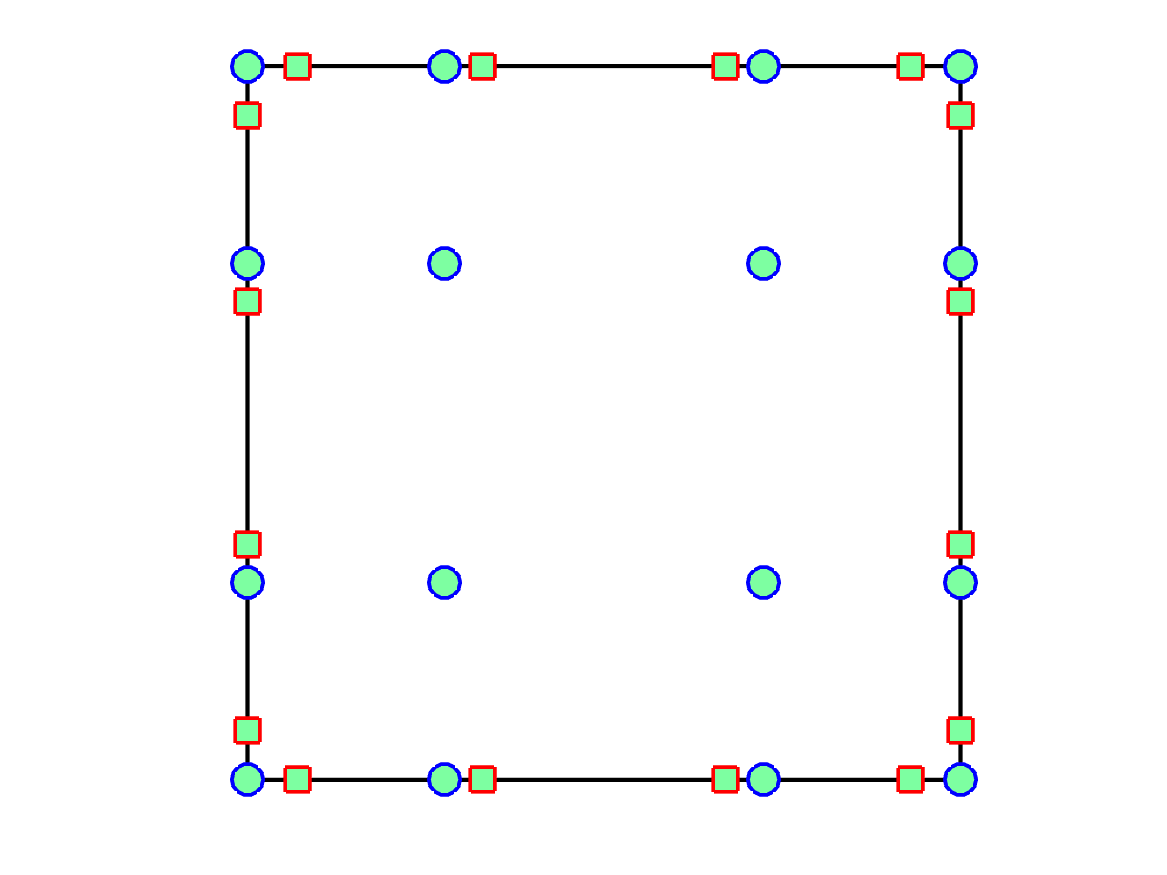
\includegraphics[width=.4\textwidth]{figs/gllgauss.png}\label{subfig:gllgq}}
\hspace{2em}
\subfloat[Degree $2N$ volume quadrature, GLL surface quadrature]{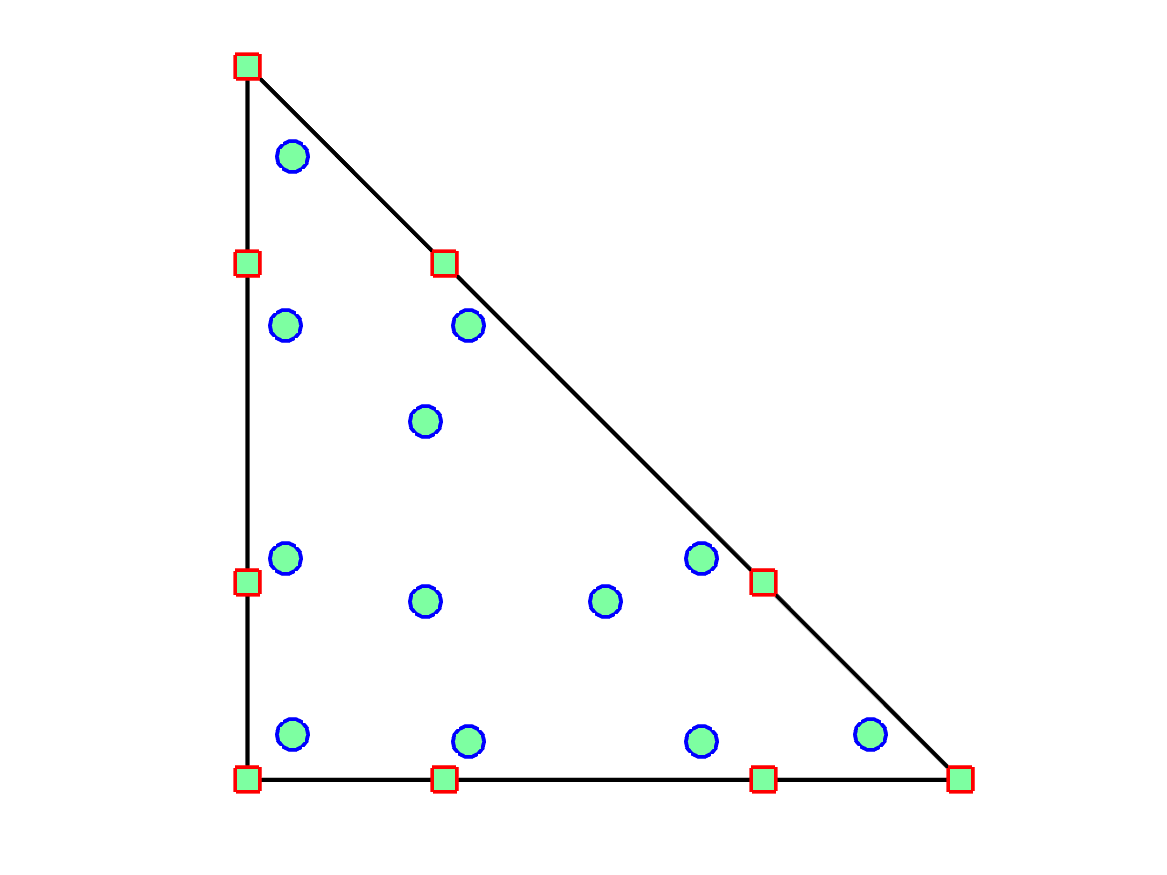
\includegraphics[width=.4\textwidth]{figs/trigll.png}\label{subfig:trigll}}
\caption{Volume and surface quadrature pairs which do not satisfy the assumptions of Theorem~\ref{lemma:dsbp}, and thus do not possess the decoupled SBP property (\ref{eq:dsbp}). Volume quadrature nodes are drawn as circles, while surface quadrature nodes are drawn as squares.}
\label{fig:sbploss}
\end{figure}

\paragraph{Quadrilateral elements (Figure~\ref{subfig:gllgq})} We first consider a quadrilateral element $\hat{D}$ with an $(N+1)$ point tensor product GLL volume quadrature and $(N+1)$ point Gauss quadrature on each face.  Let $u,v \in Q^N$ denote two arbitrary degree $N$ polynomials.  The assumptions of Theorem~\ref{lemma:dsbp} are that the volume quadrature exactly integrates $\int_{\hat{D}} \pd{u}{x_j} v$ and that the surface quadrature exactly integrates $\int_{\partial \hat{D}} u v \hat{n}_j$ on $\hat{D}$.  Because the $(N+1)$-point Gauss rule is exact for polynomials of degree $2N+1$ and the product $uv \in P^{2N}$ on each face, the surface quadrature satisfies the assumptions of Theorem~\ref{lemma:dsbp}.  However, the 1D GLL rule is only exact for polynomials of degree $(2N-1)$.  The derivative $\pd{u}{x}$ is a polynomial of degree $(N-1)$ in $x$, but is degree $N$ in $y$.  Thus, $\pd{u}{x}v$ is a polynomial of degree $(2N-1)$ in $x$ but degree $2N$ in $y$, and is not integrated exactly by the volume quadrature.  

\paragraph{Triangular elements (Figure~\ref{subfig:trigll})} We next consider a triangular element $\hat{D}$, where the volume quadrature is exact for degree $2N$ polynomials \cite{xiao2010quadrature} and an $(N+1)$-point GLL quadrature on each face.  Let $u,v \in P^N$ denote two arbitrary degree $N$ polynomials.  The derivative $\pd{u}{x} \in P^{(N-1)}$, and $\pd{u}{x}v \in P^{(2N-1)}$, so the volume quadrature satisfies the assumptions of Theorem~\ref{lemma:dsbp}.  However, because the surface quadrature is exact only degree $(2N-1)$ polynomials and the trace of $uv\in P^{2N}$, the surface quadrature does not satisfy the assumptions of Theorem~\ref{lemma:dsbp}.

\begin{figure}
\centering
\begingroup
\captionsetup[subfigure]{width=.425\textwidth}
\subfloat[Insufficiently accurate surface quadrature on the triangle element.]{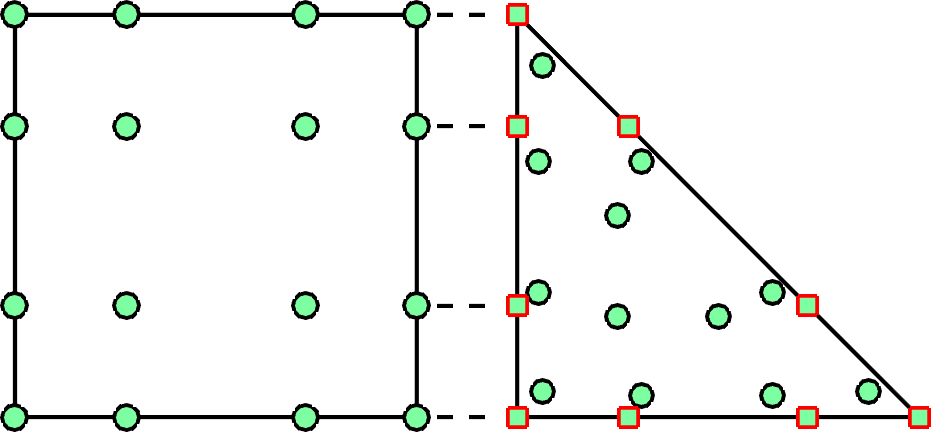
\includegraphics[width=.425\textwidth]{figs/hybrid2D.png}\label{subfig:hybrid1}}
\endgroup
\hspace{2em}
\subfloat[Incompatible surface quadrature on the quadrilateral element.]{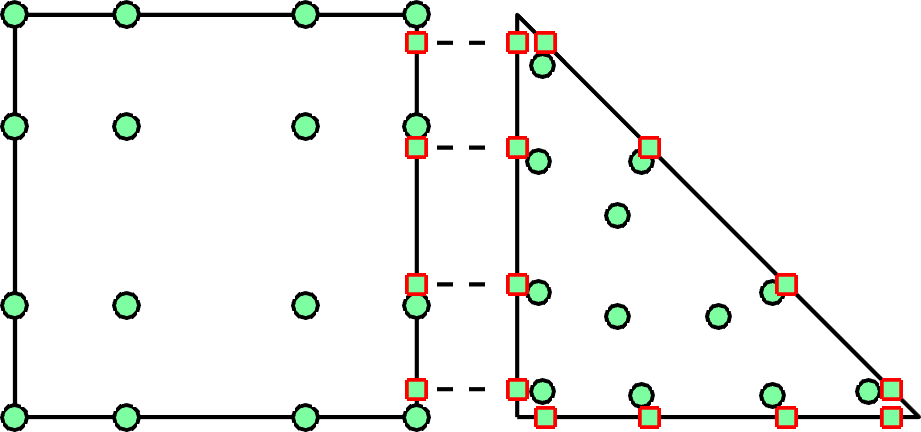
\includegraphics[width=.425\textwidth]{figs/hybrid2D_GQ.png}\label{subfig:hybrid2}}
\caption{Examples of interface couplings which do not result in a decoupled SBP property (\ref{eq:dsbp}). Volume quadrature nodes are drawn as circles, while surface quadrature nodes are drawn as  squares. }
\label{fig:hybrid}
\end{figure}

\paragraph{}These specific pairings of volume and surface quadratures appear naturally for hybrid meshes consisting of DG-SEM quadrilateral elements (using GLL volume quadrature) and triangular elements, as shown in Figure~\ref{fig:hybrid}.  In Figure~\ref{subfig:hybrid1}, the surface quadrature is a $(N+1)$ point GLL rule, and results in a loss of the SBP property on the triangle.  In Figure~\ref{subfig:hybrid2}, the surface quadrature is a $(N+1)$ point Gauss-Legendre rule, and results in a loss of the SBP property on the quadrilateral element.  The goal of this work is to construct high order accurate discretizations which preserve entropy conservation for situations in which the decoupled SBP property (\ref{eq:dsbp}) does not hold.  

%\begin{figure}
%\centering
%\subfloat[Hex-pyramid coupling]{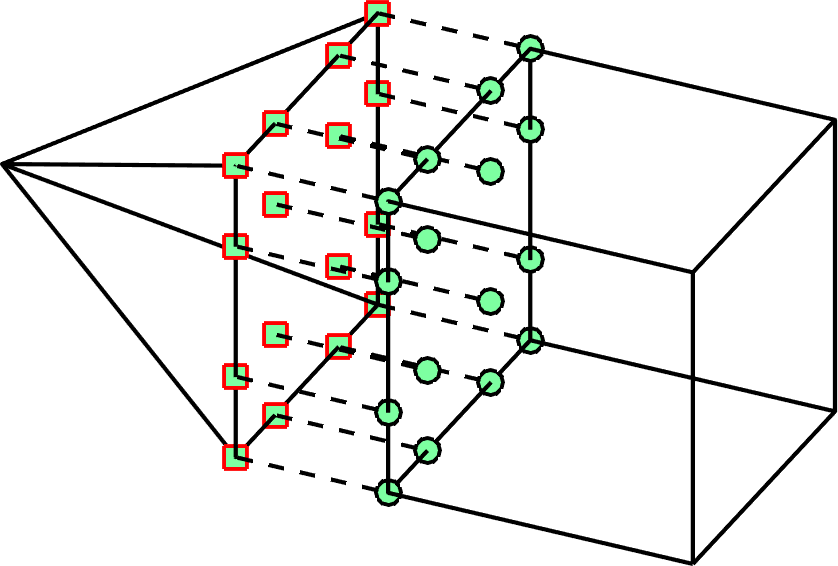
\includegraphics[width=.35\textwidth]{figs/hybrid3D.png}}
%\hspace{2em}
%\subfloat[Hex-prism coupling]{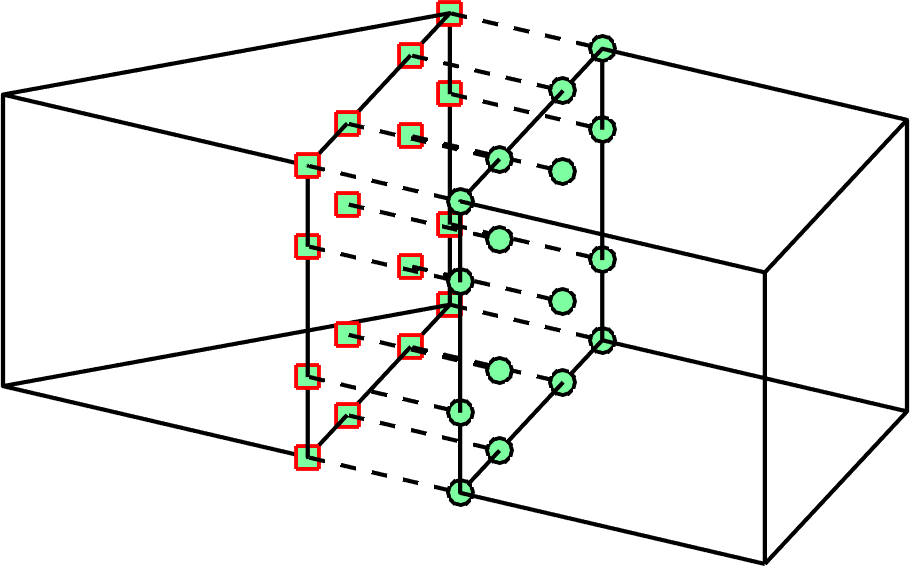
\includegraphics[width=.375\textwidth]{figs/hybrid3D_wedge.png}}
%\caption{Illustration of a 3D coupling between a GLL hexahedral element and a pyramid.  The SBP property does not hold on the pyramid due to the use of GLL quadrature on the quadrilateral face. }
%\label{fig:hybrid3d}
%\end{figure}
%
%\begin{figure}[!h]
%\centering
%\begingroup
%\captionsetup[subfigure]{width=.45\textwidth}
%\subfloat[Entropy stable inter-element coupling in \cite{friedrich2017entropy} for a non-conforming interface.]{\raisebox{0em}{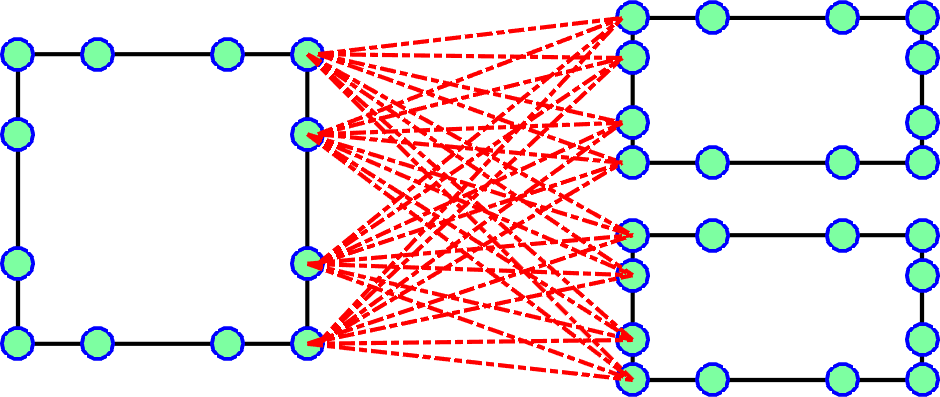
\includegraphics[width=.45\textwidth]{figs/nonconSBP.png}}\label{subfig:noncon2}}
%\hspace{2em}
%\subfloat[Entropy stable inter-element coupling in this work for a non-conforming interface.  The dotted black lines denote communication between neighboring elements.]{\raisebox{-0em}{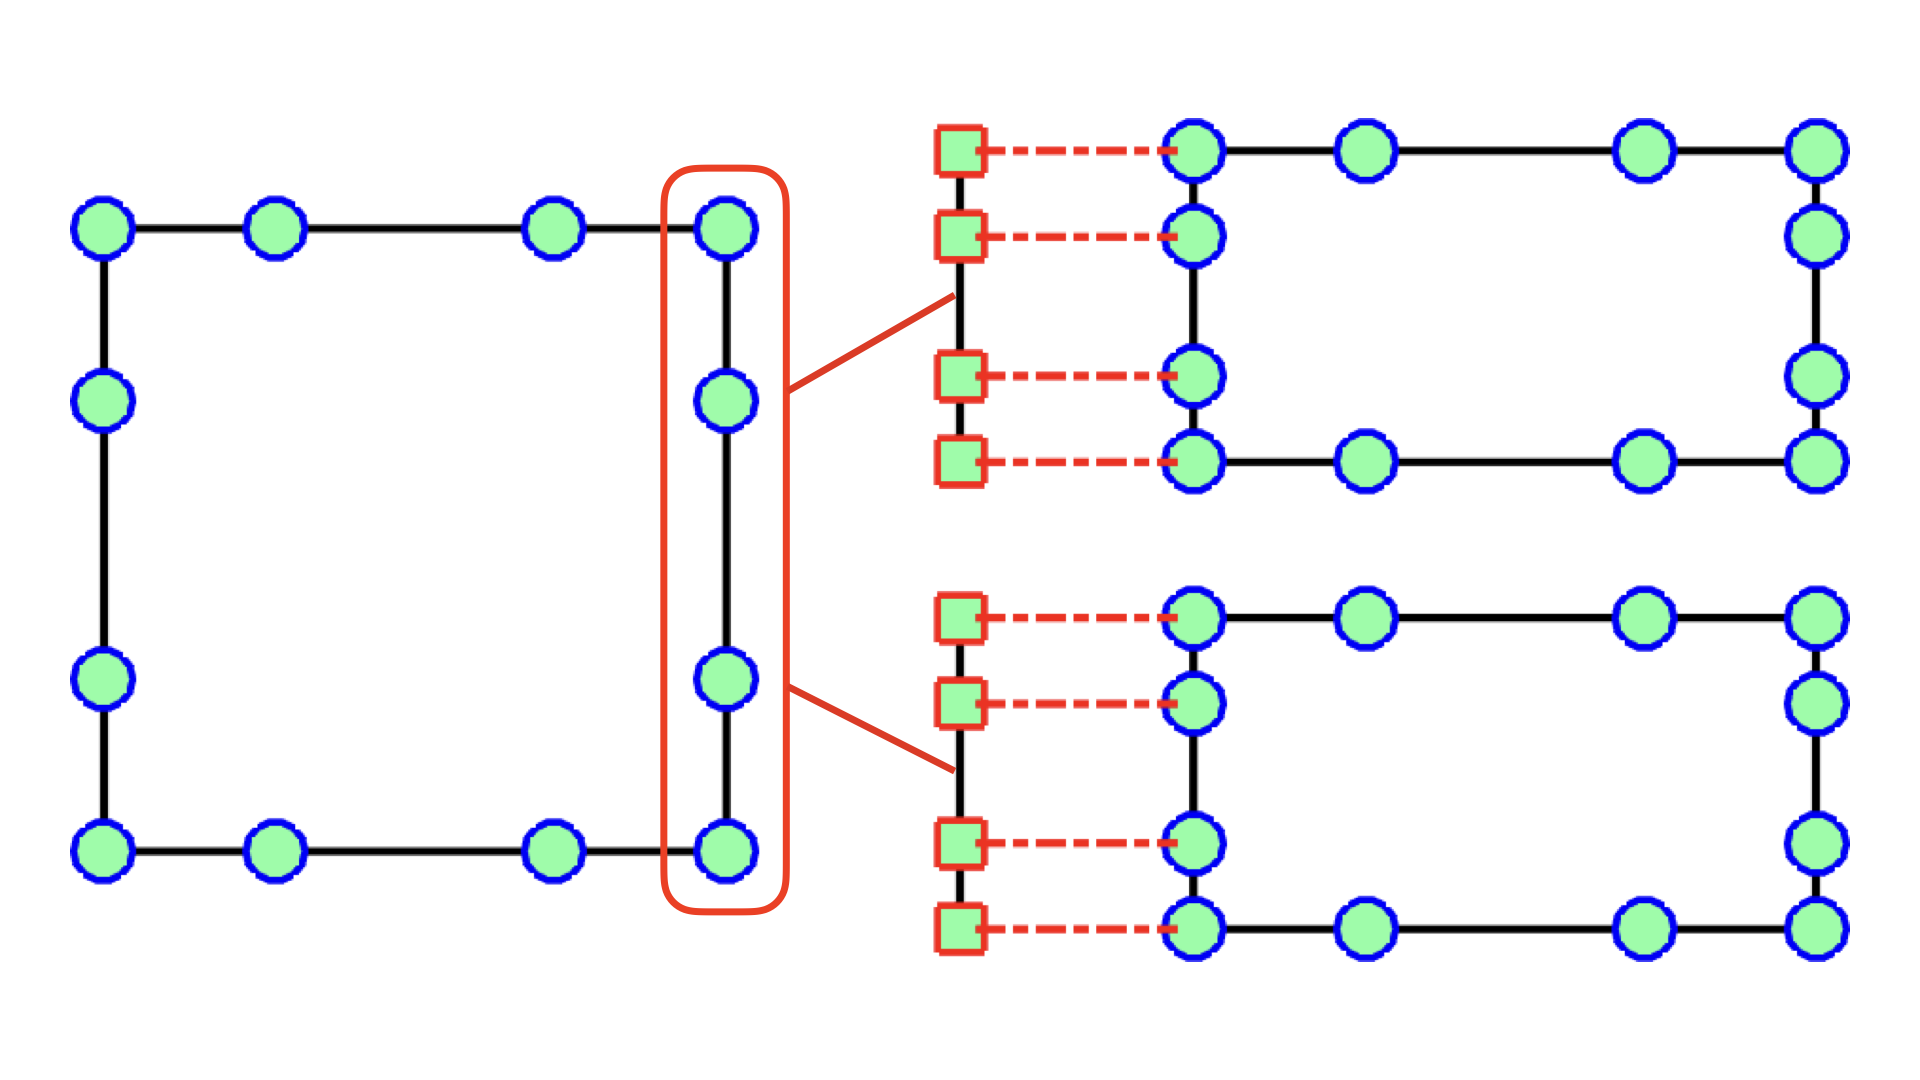
\includegraphics[width=.45\textwidth]{figs/nonconQuad.png}}\label{subfig:noncon1}}
%\endgroup
%%\subfloat[3D hexahedra-pyramid coupling]{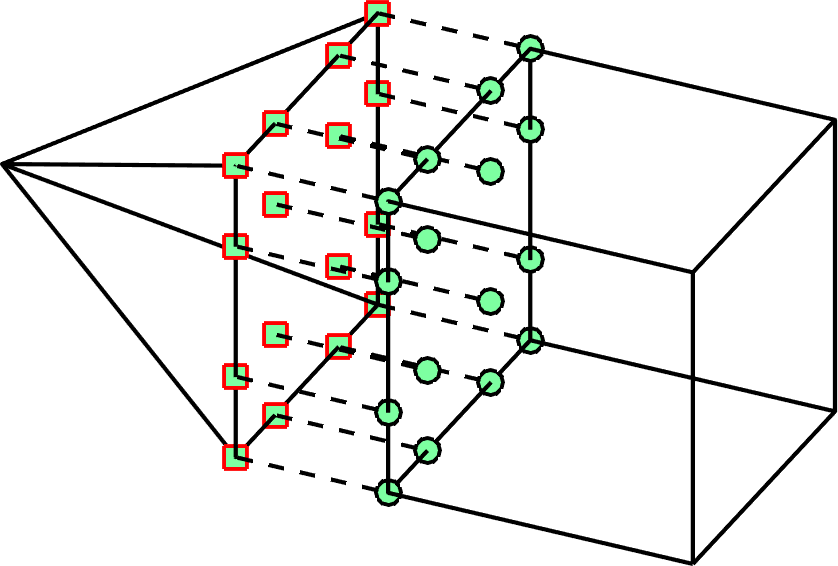
\includegraphics[width=.31\textwidth]{figs/hybrid3D.png}}
%\caption{Illustration of two different entropy stable inter-element couplings for $h$ non-conforming meshes.  Each dashed red line indicates a dyadic flux computation required between two nodes. } %The coupling terms in \cite{friedrich2017entropy} requires computing dyadic fluxes between \emph{each} pair of nodes on adjacent interfaces.  The new approach results in a simpler communication pattern between elements. }
%\label{fig:noncon}
%\end{figure}


\subsection{A variational SBP property}

%The main restriction we wish to overcome 

The property (\ref{eq:dsbp}) (which we will refer to as the ``strong'' SBP property) relates the polynomial exactness of specific quadrature rules to algebraic properties of quadrature-based matrices.  We will relax accuracy conditions on these quadrature rules by utilizing a weaker ``variational'' version of the SBP property variational, which relies on the exactness of volume and surface quadrature rules only for specific polynomials.  

On tensor product elements, we restrict ourselves to isotropic volume quadrature rules which are construced from tensor products of one-dimensional quadrature formulas.  For the remainder of this work, the degree of the multi-dimensional quadrature rule on tensor product elements will refer to the degree of exactness of the one-dimensional rule.  For example, we refer to the quadrature rule constructed through a tensor product of one-dimensional $(N+1)$-point GLL quadrature rules as a degree $(2N-1)$ quadrature rule.  This choice of quadrature is sufficient to guarantee that the mass matrix is positive definite \cite{canuto2007spectral}.  

Throughout the remainder of this work, we make the following assumptions:
\begin{assumption}
\label{ass:quad}
Let $v \in V^{N}$ denote some fixed polynomial.  We assume that: 
\begin{enumerate}
\item the mass matrix $\bm{M}$ is positive definite under the volume quadrature rule,
\item the volume quadrature rule is exact for integrals of the form\\$\int_{\hat{D}} \pd{u}{\hat{x}_j} v$ for all $u \in V^N\LRp{\hat{D}}$, $j = 1,\ldots, d$.
\item the surface quadrature rule is exact for integrals of the form\\$\int_{\partial \hat{D}} u v \hat{n}_j$ for all $u \in V^N\LRp{\hat{D}}$, $j = 1,\ldots, d$, and $f \in \partial \hat{D}$.  
\end{enumerate}
\end{assumption}

The conditions of Assumption~\ref{ass:quad} are relatively standard within the SBP literature \cite{hicken2016multidimensional, chan2017discretely, crean2018entropy}, though they have not previously depended on the specific choice of polynomial $v(\bm{x})$.   The strong SBP property (\ref{eq:dsbp}) can be derived if Assumption~\ref{ass:quad} is satisfied for all $v \in V^N$.  In contrast, we will derive a weaker SBP property which assumes only that Assumption~\ref{ass:quad} holds for a few specific polynomials $v$.  In Sections~\ref{sec:singleelem} and \ref{sec:curved}, specific polynomials $v$ will be motivated by proofs of entropy stability, and we will present examples of volume and surface quadrature rules on simplicial and tensor product elements which satisfy Assumption~\ref{ass:quad} for these choices of $v$.  
% the quantities $\int_{\hat{D}} \pd{u}{x_i} v$ and

%This section presumes that Assumption~\ref{ass:quad} is satisfied for general  $M_{\rm vol}, M_{\rm surf}$.  In Sections~\ref{sec:singleelem} and \ref{sec:curved}, specific values of $M_{\rm vol}, M_{\rm surf}$ will be motivated by proofs of entropy stability, and Assumption~\ref{ass:quad} will be verified for specific choices of volume and surface quadrature on simplicial and tensor product elements.

The conditions of Assumption~\ref{ass:quad} imply the following variational SBP property:
\begin{lemma}
\label{lemma:vsbp}
%Assume that $v \in V^M$.  
%If the volume quadrature is exact for polynomials of degree $N+M-1$ and the surface quadrature is exact for polynomials of degree $N+M$, 
Suppose Assumption~\ref{ass:quad} holds for $v(\bm{x})\in V^N$, and let $\bm{v}_q$ denote the vector of values of $v(\bm{x})$ of at volume quadrature points. Let $u(\bm{x})$ be an $L^2$ integrable function, and let $\bm{u}_q$ denote the values of $u(\bm{x})$ at quadrature points.  Then, 
\[
\bm{v}_q^T\bm{Q}_i \bm{u}_q = \bm{v}_q^T\LRp{ {\bm{E}}^T \bm{B}^i\bm{E} - \bm{Q}_i^T}\bm{u}_q.
\]
\end{lemma}
\begin{proof}
Recall that $\bm{Q}_i = \bm{W} \bm{V}_q \bm{D}^i\bm{P}_q$.  The quadrature-based $L^2$ projection $\Pi_Nu$ is a polynomial of degree $N$, and is computed discretely as $\bm{P}_q\bm{u}_q$.  By the exactness of the volume quadrature in Assumption~\ref{ass:quad}, 
\begin{align*}
\bm{v}_q^T\bm{Q}_i \bm{u}_q &= \bm{v}_q^T\bm{W} \bm{D}^i \bm{P}_q \bm{u}_q = \int_{\hat{D}} \pd{\Pi_N u}{\hat{x}_i} v = \int_{\partial \hat{D}} (\Pi_N u) v \hat{n}_i - \int_{\hat{D}} \LRp{\Pi_N u} \pd{v}{\hat{x}_i}.
\end{align*}
%Since the volume integrand $\LRp{\Pi_N u} \pd{v}{\hat{x}_i} \in V^{N+M-1}$, it is exactly integrated using the volume quadrature.  
%Additionally, since $\Pi_N u \in V^N$ and $v\in V^M$ on the surface of $\hat{D}$, the surface quadrature is exact for the surface integral and 
By the exactness of the surface quadrature in Assumption~\ref{ass:quad}, 
\begin{align*}
\int_{\partial \hat{D}} (\Pi_N u) v \hat{n}_i -   \int_{\hat{D}} \LRp{\Pi_N u} \pd{v}{\hat{x}_i} &=\bm{v}_f^T\bm{B}^i \bm{E}\bm{u}_q - \LRp{\bm{V}_q\bm{D}^i\bm{P}_q\bm{v}_q}^T\bm{W} \bm{V}_q\bm{P}_q\bm{u}_q\\
=& \bm{v}_q^T {\bm{E}}^T\bm{B}^i \bm{E}\bm{u}_q - \bm{v}_q^T \bm{P}_q^T\LRp{\bm{D}^i}^T \bm{V}_q^T \bm{W} \bm{V}_q\bm{P}_q\bm{u}_q,
\end{align*}
where we have used that, since $v \in V^N$, $\bm{v}_f = \bm{V}_f\bm{P}_q\bm{v}_q = \bm{E}\bm{v}_q$.  The proof is completed by noting that 
\[
\bm{P}_q^T\LRp{\bm{D}^i}^T \bm{V}_q^T \bm{W} \bm{V}_q\bm{P}_q = \bm{P}_q^T\LRp{\bm{D}^i}^T \bm{M}\bm{P}_q = \bm{P}_q^T\LRp{\bm{D}^i}^T \bm{V}_q^T\bm{W} = \bm{Q}_i^T.
\]
\end{proof}

The variational SBP property in Lemma~\ref{lemma:vsbp} can be used to prove a similar property for the decoupled SBP operator.  This property, along with the exact differentiation of constants, is necessary for the proof of entropy stability.  
\begin{lemma}
Suppose Assumption~\ref{ass:quad} holds.  Let $\bm{D}^i_N$ be a decoupled SBP operator on the reference element $\hat{D}$.  
%Let the volume quadrature be exact for polynomials of degree $N+M-1$, and let the surface quadrature be exact for polynomials of degree $N+M$ for some $M \leq N$.  Suppose $v\in V^N$ and that $\LRl{v}_{\partial \hat{D}} \in P^M\LRp{\partial \hat{D}}$.  \note{Fix this to match assumptions in previous lemma.}
Then, the following variational SBP property holds:
\[
\bm{v}^T\bm{Q}^i_N\bm{u} = \bm{v}^T\LRp{\bm{B}^i_N - \LRp{\bm{Q}^i_N}^T}\bm{u}.%, \qquad \bm{Q}^i_N \bm{1} = \bm{0}.
\]
where $\bm{v}, \bm{u}$ denotes the values of $v$ and $u$ at both volume and surface quadrature points.  
\label{lemma:vdsbp}
\end{lemma}
\begin{proof}
For convenience, let $\bm{u}_q, \bm{u}_f$ and $\bm{v}_q, \bm{v}_f$ denote evaluations of $u$ and $v$ at volume and surface points, such that 
\[
\bm{u} = \begin{pmatrix} \bm{u}_q\\ \bm{u}_f\end{pmatrix}, \qquad \bm{v} = \begin{pmatrix} \bm{v}_q\\ \bm{v}_f\end{pmatrix}.  
\]
The proof of the variational summation by parts property uses the definition of $\bm{Q}^i_N$ (\ref{eq:QN}), 
\begin{align*}
\bm{v}^T\bm{Q}^i_N\bm{u} &= \bm{v}_q^T\bm{Q}_i \bm{u}_q - \frac{1}{2}\LRp{\bm{E}\bm{v}_q}^T\bm{B}^i \LRp{\bm{E}\bm{u}_q} + \frac{1}{2}\LRp{\bm{E}\bm{v}_q}^T\bm{B}^i \bm{u}_f\\
& - \frac{1}{2}\bm{v}_f^T\bm{B}^i \LRp{\bm{E}\bm{u}_q} + \frac{1}{2}\bm{v}_f^T\bm{B}^i \bm{u}_f.
\end{align*}
Applying Lemma~\ref{lemma:vsbp} then yields
\begin{align*}
\bm{v}^T\bm{Q}^i_N\bm{u} =& -\bm{v}_q^T\bm{Q}^T_i \bm{u}_q + \frac{1}{2}\LRp{\bm{E}\bm{v}_q}^T\bm{B}^i \LRp{\bm{E}\bm{u}_q} + \frac{1}{2}\LRp{\bm{E}\bm{v}_q}^T\bm{B}^i \bm{u}_f\\
&\qquad - \frac{1}{2}\bm{v}_f^T\bm{B}^i \LRp{\bm{E}\bm{u}_q} - \frac{1}{2}\bm{v}_f^T\bm{B}^i \bm{u}_f + \bm{v}_f^T\bm{B}^i \bm{u}_f\\
=& \begin{pmatrix} \bm{v}_q\\ \bm{v}_f\end{pmatrix}^T 
\left(\begin{pmatrix}
\bm{0}& \\
& \bm{B}^i
\end{pmatrix}\right.+
\left.\begin{pmatrix}
-\bm{Q}_i^T + \frac{1}{2}{\bm{E}}^T\bm{B}^i \bm{E} & -\frac{1}{2} \LRp{\bm{B}^i \bm{E}}^T\\
\frac{1}{2}\bm{B}^i \bm{E} & -\frac{1}{2}\bm{B}^i
\end{pmatrix}  \right)
\begin{pmatrix} \bm{u}_q\\ \bm{u}_f\end{pmatrix}\\
=& \bm{v}^T\LRp{\bm{B}^i_N - \LRp{\bm{Q}^i_N}^T}\bm{u}.
\end{align*}
\end{proof}

\subsection{Entropy stability on a reference element}
\label{sec:singleelem}

In this section, we construct so-called ``entropy stable'' schemes on the reference element $\hat{D}$.  These methods ensure that the entropy inequality (\ref{eq:entropyineq}) is satisfied discretely by avoiding the use of the chain rule in the proof of entropy dissipation.  Entropy stable schemes rely on two main ingredients: an entropy stable numerical flux as defined by Tadmor \cite{tadmor1987numerical} and a concept referred to as ``flux differencing''.  Let $\bm{f}_S\LRp{\bm{u}_L,\bm{u}_R}$ be a numerical flux function which is a function of ``left'' and ``right'' states $\bm{u}_L,\bm{u}_R$.  The numerical flux $\bm{f}_S$ is \textit{entropy conservative} if it satisfies the following three conditions:  
\begin{gather}
\bm{f}^i_S(\bm{u},\bm{u}) = \bm{f}_i(\bm{u}), \qquad \text{(consistency)}\\
\bm{f}^i_S(\bm{u}_L,\bm{u}_R) = \bm{f}^i_S(\bm{u}_R,\bm{u}_R), \qquad \text{(symmetry)}\nonumber\\
\LRp{\bm{v}_L-\bm{v}_R}^T\bm{f}^i_S(\bm{u}_L,\bm{u}_R) = \psi_i(\bm{u}_L) - \psi_i(\bm{u}_R), \qquad \text{(conservation)}\nonumber
\label{eq:esflux}
\end{gather}
for $j = 1,\ldots, d$.  The construction of entropy stable schemes will utilize (\ref{eq:esflux}) in discretizations of both volume and surface terms in a DG formulation.  

Proving a semi-discrete entropy inequality typically involves the ``strong'' SBP condition.  The schemes presented in this work will relax this, and use only two (weaker) conditions: that the decoupled SBP operator $\bm{D}^i_N$ exactly differentiates constants and that a discrete form of the fundamental theorem of calculus (FTC) holds.  The latter property can be derived from the variational SBP property in Lemma~\ref{lemma:vdsbp}.

\begin{lemma}{(Discrete FTC and exact differentiation of constants)}
\label{lemma:sbpcor}
Suppose Assumption~\ref{ass:quad} holds for $v(\bm{x}) = 1$.  
Let $u(\bm{x})$ be some $L^2$ integrable function, and let $\bm{u}$ denote the vector of values of $u(\bm{x})$ at volume and surface quadrature points. Then, 
\[
\bm{1}^T\bm{Q}^i_N\bm{u} = \bm{1}^T\bm{B}^i_N\bm{u}, \qquad \bm{Q}^i_N\bm{1} = \bm{0}.
\]
\end{lemma}
\begin{proof}
The proof that $\bm{Q}^i_N \bm{1} = \bm{0}$ follows from the property that polynomials are equal to their $L^2$ projection, and is identical to that of \cite{chan2017discretely,chan2018discretely}.     The proof of the first equality follows from $\bm{Q}^i_N \bm{1} = \bm{0}$ and Lemma~\ref{lemma:vdsbp} 
\[
\bm{1}^T\LRp{\bm{Q}^i_N}\bm{u} = \bm{1}^T\LRp{\bm{B}^i_N - \LRp{\bm{Q}^i_N}^T}\bm{u} = \bm{1}^T{\bm{B}^i_N}\bm{u}.
\]
\end{proof}

We can now construct a skew-symmetric formulation on the reference element $\hat{D}$ and show that it is semi-discretely entropy conservative. This formulation can be made entropy stable by adding interface dissipation.  Let $\bm{u}_h$ denote the discrete solution, and let $\bm{u}_q$ denote the values of the solution at volume quadrature points.  We define the auxiliary conservative variables $\tilde{\bm{u}}$ in terms of the $L^2$ projections of the entropy variables 
\begin{gather}
\bm{v}_q = \bm{v}\LRp{\bm{u}_q}, \qquad \tilde{\bm{v}} = \begin{bmatrix}
\bm{V}_q\\
\bm{V}_f
\end{bmatrix}\bm{P}_q\bm{v}_q, \qquad \tilde{\bm{u}} = \bm{u}\LRp{\tilde{\bm{v}}}.
\end{gather}
The skew-symmetric formulation for (\ref{eq:nonlineqs}) on $\hat{D}$ is given in terms of $\tilde{\bm{u}}$
\begin{gather}
\bm{M}\pd{\bm{u}_h}{t} + \sum_{i=1}^d\LRs{\begin{array}{c}
\bm{V}_q \\ \bm{V}_f\end{array}}^T 
\LRp{\LRp{\bm{Q}^i_N - \LRp{\bm{Q}^i_N}^T} \circ \bm{F}^i_S}\bm{1} + \bm{V}_f^T\bm{B}^i\bm{f}_i^* = 0,  \label{eq:esdgSkew}\\
\LRp{\bm{F}^i_S}_{ij} = \bm{f}^i_S\LRp{\tilde{\bm{u}}_i,\tilde{\bm{u}}_j}, \qquad 1\leq i,j\leq N_q + N^f_q,\nonumber
\end{gather}
where $\bm{f}^*$ is some numerical flux, and the matrix $\LRp{\bm{Q}^i_N - \LRp{\bm{Q}^i_N}^T}$ possesses the following block structure:
\[
\LRp{\bm{Q}^i_N - \LRp{\bm{Q}^i_N}^T} = \begin{pmatrix}
\bm{Q}_i-\bm{Q}_i^T & {\bm{E}}^T \bm{B}^i\\
-\bm{B}^i\bm{E} & \bm{0}
\end{pmatrix}.
\]
Multiplying the formulation (\ref{eq:esdgSkew}) by $\bm{M}^{-1}$ on both sides yields a strong form 
\begin{gather}
\pd{\bm{u}_h}{t} + \sum_{i=1}^d \LRs{\begin{array}{cc}
\bm{P}_q & \bm{L}_f\end{array}} \LRp{\LRp{\bm{D}^i_N - \bm{W}_N^{-1}\LRp{\bm{Q}^i_N}^T} \circ \bm{F}^i_S}\bm{1} + \bm{L}_f \diag{\hat{\bm{n}}_i}\bm{f}_i^* = 0,\label{eq:esdg}
%\\
%\LRp{\bm{F}_S}_{ij} = \bm{f}_S\LRp{\tilde{\bm{u}}_i,\tilde{\bm{u}}_j}, \qquad 1\leq i,j\leq N_q + N^f_q.
%\label{eq:esdgSkewStrong}
\end{gather}
We can now show that the skew-symmetric formulation is entropy conservative.  
\begin{theorem}
Suppose Assumption~\ref{ass:quad} holds for $v(\bm{x}) = 1$.  
Then, the formulation (\ref{eq:esdgSkew}) is entropy conservative such that
\begin{equation}
\bm{1}^T\bm{W}\pd{U(\bm{u}_q)}{t} + \sum_{i=1}^d\bm{1}^T\bm{B}^i \LRp{\psi_i(\tilde{\bm{u}}_f) - \tilde{\bm{v}}_f^T\bm{f}_i^*} = 0, \qquad \bm{u}_q = \bm{V}_q\bm{u}.
\label{eq:esdgthm}
\end{equation}
\label{thm:esdg}
\end{theorem}
\begin{proof}
Testing (\ref{eq:esdgSkew}) by $\bm{v}_h = \bm{P}_q\bm{v}_q$ yields 
\begin{align}
\bm{v}_q^T\bm{W}\pd{\LRp{\bm{V}_q\bm{u}}}{t} + \sum_{i=1}^d
\tilde{\bm{v}}^T \LRp{\LRp{\bm{Q}^i_N - \LRp{\bm{Q}^i_N}^T} \circ \bm{F}^i_S}\bm{1} + \tilde{\bm{v}}_f^T \bm{B}^i\bm{f}_i^* = 0.
\end{align}
One can show that \cite{chan2017discretely}
\begin{align*}
\tilde{\bm{v}}^T \LRp{\LRp{\bm{Q}^i_N - \LRp{\bm{Q}^i_N}^T} \circ \bm{F}^i_S}\bm{1} &= \tilde{\bm{v}}^T \LRp{\bm{Q}^i_N \circ \bm{F}^i_S}\bm{1} - \tilde{\bm{v}}^T \LRp{\LRp{\bm{Q}^i_N}^T \circ \bm{F}^i_S}\bm{1}\\
&= \tilde{\bm{v}}^T \LRp{\bm{Q}^i_N \circ \bm{F}^i_S}\bm{1} - \bm{1}^T \LRp{{\bm{Q}^i_N} \circ \bm{F}^i_S}\tilde{\bm{v}}.
\end{align*}
Where we have used that $\bm{F}^i_S$ is symmetric and that the Hadamard product commutes.  Applying the conservation condition on $\bm{f}^i_S$ in (\ref{eq:esflux}) then yields
\begin{align*}
&\tilde{\bm{v}}^T \LRp{\bm{Q}^i_N \circ \bm{F}^i_S}\bm{1} - \bm{1}^T \LRp{{\bm{Q}^i_N} \circ \bm{F}^i_S}\tilde{\bm{v}} \\
&= \sum_{jk} \LRp{\bm{Q}^i_N}_{jk} \LRp{\tilde{\bm{v}}_j-\tilde{\bm{v}}_k} \bm{f}_S\LRp{\tilde{\bm{u}}_j,\tilde{\bm{u}}_k} = \sum_{jk} \LRp{\bm{Q}^i_N}_{jk} \LRp{\psi_i(\tilde{\bm{u}}_j) - \psi_i(\tilde{\bm{u}}_k)}\\
&= \bm{1}^T\LRp{\bm{Q}^i_N}\psi_i(\tilde{\bm{u}}) - \psi_i(\tilde{\bm{u}})^T\LRp{\bm{Q}^i_N}\bm{1} = \bm{1}^T\LRp{\bm{Q}^i_N}\psi_i(\tilde{\bm{u}}) = \bm{1}^T\bm{B}^i_N\psi_i(\tilde{\bm{u}}),
\end{align*}
where we have used Lemma~\ref{lemma:sbpcor} in the last equality.  Noting that $\bm{1}^T\bm{B}^i_N\psi_i(\tilde{\bm{u}}) = \bm{1}^T\bm{B}^i \psi_i(\tilde{\bm{u}}_f)$ completes the proof.
%The final step of the proof is  where we have used Lemma~\ref{lemma:vdsbp} to integrate by parts and conclude that $\bm{1}^T\LRp{\bm{Q}^i_N}^T = 0$.
\end{proof}

\begin{remark}
The primary difference between this formulation and the formulation presented in \cite{chan2017discretely} is the use of the skew-symmetric volume operator $\LRp{\bm{Q}^i_N - \LRp{\bm{Q}^i_N}^T}$.  When the strong SBP property (\ref{eq:dsbp}) holds, this formulation is exactly equivalent to the strong formulation presented in \cite{chan2017discretely}.  However, the only result necessary to prove Theorem~\ref{thm:esdg} is Lemma~\ref{lemma:sbpcor}.  The decoupled SBP property (\ref{eq:dsbp}) is not utilized, and is not necessary to guarantee a semi-discrete conservation of entropy for the skew-symmetric formulation.  
\end{remark}


The skew symmetric formulation can also be shown to be locally conservative in the sense of \cite{shi2017local}, which is sufficient to show the numerical solution convergences to the weak solution under mesh refinement.  
\begin{theorem}
The formulation (\ref{eq:esdgSkew}) is locally conservative such that
\begin{align}
\bm{1}^T\bm{W}\pd{\LRp{\bm{V}_q\bm{u}}}{t} + \sum_{i=1}^d\bm{1}^T\bm{B}^i\bm{f}_i^* = 0. 
\end{align}
\end{theorem}
\begin{proof}
To show local conservation, we test (\ref{eq:esdgSkew}) with $1$
\begin{align}
\bm{1}^T\bm{W}\bm{V}_q\pd{\bm{u}_h}{t} + \sum_{i=1}^d
\bm{1}^T
\LRp{\LRp{\bm{Q}^i_N - \LRp{\bm{Q}^i_N}^T} \circ \bm{F}_S}\bm{1} + \bm{1}^T\bm{W}_f \diag{\hat{\bm{n}}}\bm{f}_i^* = 0. 
\end{align}
Because $\bm{F}_S$ is symmetric and $\LRp{\bm{Q}^i_N - \LRp{\bm{Q}^i_N}^T}$ is skew-symmetric, their Hadamard product is also skew-symmetric.  Using that $\bm{x}^T\bm{A}\bm{x} = 0$ for any skew symmetric matrix $\bm{A}$, the volume term $\bm{1}^T\LRp{\LRp{\bm{Q}^i_N - \LRp{\bm{Q}^i_N}^T} \circ \bm{F}_S}\bm{1}$ vanishes.
% and that the Hadamard product is commutable $\LRp{\bm{A}\circ\bm{B} }^T = \bm{A}^T\circ\bm{B}^T$
%\begin{align}
%\bm{1}^T\LRp{\LRp{\bm{Q}^i_N - \LRp{\bm{Q}^i_N}^T} \circ \bm{F}_S}\bm{1} &= \bm{1}^T\LRp{\bm{Q}^i_N\circ \bm{F}_S}\bm{1} - \bm{1}^T\LRp{\LRp{\bm{Q}^i_N}^T\circ \bm{F}_S}\bm{1}\\
%&= \bm{1}^T\LRp{\bm{Q}^i_N\circ \bm{F}_S}\bm{1} - 
%\bm{1}^T\LRp{\bm{Q}^i_N\circ \bm{F}_S}\bm{1} = 0,
%\end{align}
%where we have used that $\bm{F}_S$ is symmetric.
%\begin{align}
%\end{align}
\end{proof}

\subsection{On quadrature conditions for Assumption~\ref{ass:quad} with $v = 1$}
\label{sec:assump1}
Apart from algebraic manipulations, only Lemma~\ref{lemma:sbpcor} is necessary to prove entropy conservation for (\ref{eq:esdg}).  Lemma~\ref{lemma:sbpcor} requires that Assumption~\ref{ass:quad} holds for $v=1$.  Thus, the volume and surface quadratures must be sufficiently accurate to guarantee that the mass matrix is positive definite and to integrate 
\begin{equation}
\int_{\hat{D}} \pd{u}{x_i}, \qquad \int_{\partial \hat{D}} u \hat{n}_i. \label{eq:affineints}
\end{equation}
On simplicial elements, the mass matrix is guaranteed to be positive definite for any volume quadrature which is exact for degree $2N$ polynomial integrands.  This choice of volume quadrature also guarantees that the volume term in (\ref{eq:affineints}) is integrated exactly.  The surface quadrature can thus be taken to be any quadrature rule which is exact for only degree $N$ integrands on faces.  In contrast, the construction of simplicial decoupled SBP operators has required face quadratures which are accurate for degree $2N$ polynomials \cite{chan2017discretely, chan2018discretely}.  

On tensor product elements, we can take any degree $(2N-1)$ quadrature rule which ensures a positive definite mass matrix (e.g.\ a $(N+1)$-point GLL quadrature), as a quadrature of this accuracy is sufficient to exactly integrate the volume term in (\ref{eq:affineints}).  For the surface quadrature, we can again take any quadrature rule which is exact for degree $N$ polynomial integrands.  For example, on a quadrilateral element, one can use $\left\lceil\frac{N+1}{2}\right\rceil$-point Gauss quadrature rule or a $\left\lceil\frac{N+3}{2}\right\rceil$-point GLL rule as face quadratures for a degree $N$ scheme.  

%\note{link SBP accuracy section} %These issues will be discussed further in Section~\ref{sec:num}.
%This minimal degree of surface quadrature accuracy will depend on the nature of the physical mesh, and will differ between affine and curved elements.  

\section{Skew-symmetric entropy conservative formulations on mapped elements}
\label{sec:skew2}

We now construct skew-symmetric formulations on mapped elements.  We assume some domain $\Omega$ is decomposed into non-overlapping elements $D^k$, such that $D^k$ is the image of the reference element $\hat{D}$ under an isoparametric mapping $\bm{\Phi}^k$.  We define geometric change of variables terms ${G}^k_{ij}$ as scaled derivatives of reference coordinates $\hat{\bm{x}}$ w.r.t.\ physical coordinates $\bm{x}$
\begin{gather}
\pd{u}{x_i} = \sum_{ij} {G}^k_{ij}\pd{u}{\hat{x}_j}, \qquad {G}^k_{ij} = J^k\pd{\hat{x}_j}{{x}_i}, 
\label{eq:geofacs}
\end{gather}
where $J^k$ is the determinant of the Jacobian of the geometric mapping on the element $D^k$.  We also introduce the scaled outward normal components $n_iJ^k_f$, which can be computed in terms of (\ref{eq:geofacs}) and the reference normals $\hat{\bm{n}}$ on $\hat{D}$
\begin{gather}
n^k_i J^k_f = \sum_{j=1}^d G^k_{ij} \hat{{n}}_j.  
\label{eq:normals}
\end{gather}
We also define $\bm{n}^k_i$ as the vector containing concatenated values of the scaled outward normals $n^k_iJ^k_f$ at surface quadrature nodes.  For the remainder of the work, we assume that the mesh is watertight \cite{chan2018discretely} such that at all points on any internal face, the scaled outward normals $n^k_iJ^k_f$ on the two elements sharing this face are equal and opposite.  

%Derivatives with respect to physical coordinates on $D^k$ are computed in terms of a change of variables formula and geometric terms (\ref{eq:geofacs}).  
%%For affine meshes, the scaled geometric terms ${G}^k_{ij}$ are constant over each element.  It was shown in \cite{chan2017discretely} that one can define a physical differentiation matrix as a linear combination of reference differentiation matrices.  
%Let ${\bm{D}}^i_N$ denote the decoupled SBP operator on the reference element $\hat{D}$.  Define the decoupled SBP operators $\bm{D}^i_k$ with respect to the physical coordinates on $D^k$ be defined as
%\begin{align}
%{\bm{D}}^i_k = \sum_{j=1}^d {G}^k_{ij}\hat{\bm{D}}^j_N.
%\end{align}

%\note{Maybe remove affinely mapped elements section.}  
%
%\subsection{Affinely mapped elements}
%\label{sec:affine}
%
%We first extend this formulation to affinely mapped elements.  Let the domain be 
%
%Let Assumption~\ref{ass:quad} again hold for $v(\bm{x}) = 1$.  Then, it is straightforward to show that the following formulation on $D^k$ is locally entropy conservative: 
%\begin{gather}
%J^k\bm{M}\pd{\bm{u}_h}{t} + 
%\sum_{i=1}^d \LRs{\begin{array}{cc}
%\bm{V}_q \\
%\bm{V}_f\end{array}}^T \LRp{\LRp{\bm{Q}^i_k - \LRp{\bm{Q}^i_k}^T} \circ \bm{F}_S}\bm{1} + \bm{V}_f^T\bm{W}_f \diag{{\bm{n}^k_i}}\bm{f}_i^* = 0, \label{eq:skewform}\\
%%\sum_{i=1}^d \LRs{\begin{array}{cc}
%%\bm{P}_q & \bm{L}_f\end{array}} \LRp{\LRp{\bm{D}^i_N - \bm{W}_N^{-1}\LRp{\bm{Q}^i_N}^T} \circ \bm{F}_S}\bm{1} + \bm{L}_f \diag{{\bm{n}_i}}\bm{f}_i^* = 0, \label{eq:skewform}\\
%\LRp{\bm{F}_S}_{ij} = \bm{f}_S\LRp{\tilde{\bm{u}}_i,\tilde{\bm{u}}_j}, \qquad 1\leq i,j\leq N_q + N^f_q, \nonumber\\
%\bm{f}^* = \bm{f}_S(\tilde{\bm{u}}_f^+,\tilde{\bm{u}}_f), \qquad \text{ on interior interfaces,} \nonumber
%\end{gather}
%where $\tilde{\bm{u}}_f^+$ denotes the face value of the entropy-projected conservative variables $\tilde{\bm{u}}_f$ on the neighboring element.  The proof of global entropy conservation follows as in \cite{chan2017discretely}, and results from summing up (\ref{eq:esdgthm}) over all elements and noting that the surface terms cancel due to the symmetry and conservation properties of the Tadmor flux (\ref{eq:esflux}).  The entropy conservative formulation (\ref{eq:skewform}) can be made entropy stable by adding appropriate interface dissipation, such as Lax-Friedrichs or matrix-based penalization terms \cite{winters2017uniquely, chen2017entropy, chan2017discretely}.  


%On affine meshes, it is possible to show entropy stability of the skew-symmetric formulation (\ref{eq:esdgSkew}) under a surface quadrature which is only exact for degree $N$ polynomials.  
On a single element (and on affine meshes), it is possible to show entropy stability of the skew-symmetric formulation (\ref{eq:esdgSkew}) under a surface quadrature which is only exact for degree $N$ polynomials.  However, on curved meshes, stronger conditions are required to guarantee entropy stability.  This is due to the fact that the geometric terms are now high order polynomials which vary spatially over each element.  Moreover, Lemma~\ref{lemma:sbpcor} assumes affine geometric mappings, and does not hold on curved elements.  In this section, we discuss how to extend Lemma~\ref{lemma:sbpcor} to curved simplicial and tensor product elements.  

\subsection{Curved elements and the geometric conservation law}
\label{sec:curved}

%Let the domain now be triangulated by a  consisting of curved elements $D^k$.  
In this section, we describe how to construct appropriate decoupled SBP operators on curved meshes, and give conditions on the volume and surface quadrature rules under which a semi-discretely entropy stable scheme can be constructed.

%For a curved element $D^k$, geometric terms $G^k_{ij}$ are high order polynomials over the reference domain $\hat{D}$.  

We first show how to construct decoupled SBP operators on curved elements.  Let $\bm{G}^k_{ij}$ denote the vector of scaled geometric terms ${G}^k_{ij}$ evaluated at both volume and surface quadrature points, and let $\hat{\bm{D}}^j_N$ denote the decoupled SBP operator for the $j$th reference coordinate.  Decoupled SBP operators on a curved element $D^k$ can be defined as in \cite{chan2018discretely} by
\begin{equation}
\bm{D}^i_k = \frac{1}{2}\sum_{j=1}^d \LRp{\diag{\bm{G}^k_{ij}}\hat{\bm{D}}^j_N + \hat{\bm{D}}^j_N\diag{\bm{G}^k_{ij}}}, \qquad \bm{Q}^i_k = \bm{W} \bm{D}^i_k.
\label{eq:dncurved}
\end{equation}
It can be shown that, if $\hat{\bm{D}}^j_N$ satisfies a strong summation by parts property, $\bm{D}^i_k$ satisfies an analogous strong summation by parts property.

For curved elements, steps must also be taken to ensure that the analogue of Lemma~\ref{lemma:vdsbp} and Lemma~\ref{lemma:sbpcor} hold at the discrete level.  Expanding out the condition $\bm{Q}^i_k\bm{1} = \bm{0}$ in terms of (\ref{eq:dncurved}) yields
\begin{align}
\bm{Q}^i_k \bm{1} = \frac{1}{2} \bm{W}\sum_{j=1}^d \diag{\bm{G}^k_{ij}}\hat{\bm{D}}^j_N \bm{1} + \hat{\bm{D}}^j_N\diag{\bm{G}^k_{ij}}\bm{1} = \frac{1}{2}\bm{W}\sum_{j=1}^d \hat{\bm{D}}^j_N\LRp{\bm{G}^k_{ij}} = 0,
\label{eq:dgcl}
\end{align}
where we have used that $\hat{\bm{D}}^j_N \bm{1} = 0$.  We refer to the condition $\bm{Q}^i_k\bm{1} = 0$ as the discrete geometric conservation law (GCL) \cite{thomas1979geometric, kopriva2006metric}.  For degree $N$ isoparametric mappings, the GCL is automatically satisfied in two dimensions due to the fact that the exact geometric terms ${G}^k_{ij}$ are polynomials of degree $N$ \cite{kopriva2006metric}.  However, in three dimensions, the GCL is not automatically satisfied due to the fact that the degree of $G^k_{ij}$ is larger than $N$.  Thus, the geometric terms cannot be represented exactly using degree $N$ polynomials, and (\ref{eq:dgcl}) must be enforced through an alternative construction of ${G}^k_{ij}$.  

A common approach is to rewrite the geometric terms as the curl of some quantity $\bm{r}^i$, but to interpolate $\bm{r}^i$ before applying the curl \cite{visbal2002use, kopriva2006metric, hindenlang2012explicit, chan2018discretely}:
\begin{gather}
\bm{r}^i = { \pd{\bm{x}}{\hat{x}_i}\times \bm{x}}, \qquad
\LRs{\begin{array}{c}
{G}^k_{1j}\\
{G}^k_{2j}\\
{G}^k_{3j}\end{array}} = \begin{bmatrix}
\LRp{-\hat{\Grad}\times I_{N_{\rm geo}}\LRp{x_3\hat{\Grad}x_2}}_j\\
\LRp{\hat{\Grad}\times I_{N_{\rm geo}}\LRp{x_3\hat{\Grad}x_1}}_j\\
\LRp{\hat{\Grad}\times I_{N_{\rm geo}}\LRp{x_1\hat{\Grad}x_2}}_j
\end{bmatrix},\\
%-\frac{1}{2}\LRp{\pd{I_{N_{\rm geo}}\bm{r}^k}{\hat{x}_j}-\pd{I_{N_{\rm geo}}\bm{r}^j}{\hat{x}_k}},\\
N_{\rm geo} \leq \begin{cases}
N+1 & \text{(tetrahedra)}\\
N & \text{(hexahedra)}
\end{cases},\nonumber
\label{eq:iconscurl}
\end{gather}
where $I_{N_{\rm geo}}$ denotes a degree $N_{\rm geo}$ polynomial interpolation operator with appropriate interpolation nodes.\footnote{This interpolation step must be performed using interpolation points with an appropriate number of nodes on each boundary \cite{chan2018discretely}.  These include, for example, GLL nodes on tensor product elements, as well as Warp and Blend nodes on non-tensor product elements \cite{warburton2006explicit, chan2015comparison}.}  The restriction on the maximum value of $N_{\rm geo}$ ensures that $G^k_{ij} \in V^N$ (e.g. $G^k_{ij} \in P^N$ on tetrahedral elements and $G^k_{ij}\in Q^N$ on hexahedral elements), which is also necessary to guarantee (\ref{eq:dgcl}).

Because the decoupled SBP operators $\bm{D}^i_k$ are now defined through (\ref{eq:dncurved}), Lemma~\ref{lemma:sbpcor} and the proof of entropy stability no longer hold for curved elements and must be modified.  The introduction of curvilinear meshes will impose slightly different conditions on the accuracy of the surface quadrature.  We discuss simplicial and tensor product elements separately, as differences in the natural polynomial approximation spaces will result in different assumptions for each proof.

\begin{lemma}{(Discrete FTC and exact constant differentiation on curved elements)}
\label{lemma:vdsbpcurved} 
Let $D^k$ be a curved element, and let the geometric terms $G^k_{ij}$ be constructed using (\ref{eq:iconscurl}).  Let Assumption~\ref{ass:quad} hold for $v = 1$ and $v = G^k_{ij}$ for all $i,j = 1,\ldots, d$, and let $\bm{u}$ denote a vector of values of some function at volume and surface quadrature points.  Then, 
%If the volume quadrature is exact for polynomials of degree $(N+N_{\rm geo}-1)$ and the surface quadrature is exact for polynomials of degree $(N+N_{\rm geo})$, then 
\[
\bm{1}^T\bm{Q}^i_k\bm{u} = \bm{1}^T\bm{B}^i_k\bm{u}, \qquad \bm{Q}^i_k\bm{1} = \bm{0},
\]
where the physical boundary matrix $\bm{B}^i_k$ is defined as
\[
\bm{B}^i_k = \sum_{j=1}^d \bm{B}^j_N \diag{\bm{G}^k_{ij}} = \sum_{j=1}^d \diag{\bm{G}^k_{ij}}\bm{B}^j_N  = \begin{pmatrix}
\bm{0}&\\
& \bm{W}_f \diag{\bm{n}^k_i}\end{pmatrix}.
\]
\end{lemma}
\begin{proof}
The proof of $\bm{Q}^i_k\bm{1} = \bm{0}$ was shown for for tensor product elements in \cite{kopriva2006metric} and for simplicial elements in \cite{chan2018discretely}, and relies only on the fact that $G^k_{ij} \in V^N$.  

The discrete fundamental theorem of calculus $\bm{1}^T\bm{Q}^i_k\bm{u} = \bm{1}^T\bm{B}^i_k\bm{u}$ can be shown to hold using (\ref{eq:dncurved}):
\begin{align*}
\bm{1}^T\bm{Q}^i_k\bm{u} &= \frac{1}{2}\sum_{j=1}^d \bm{1}^T{\LRp{\diag{\bm{G}^k_{ij}}\hat{\bm{Q}}^j_N + \hat{\bm{Q}}^j_N\diag{\bm{G}^k_{ij}}}} \bm{u} \\
&= \frac{1}{2}\sum_{j=1}^d \LRp{\LRp{\bm{G}^k_{ij}}^T \hat{\bm{Q}}^j_N\bm{u} + \bm{1}^T\hat{\bm{Q}}^j_N\diag{\bm{G}^k_{ij}}\bm{u}}.
\end{align*}
Applying Lemma~\ref{lemma:vdsbp} to $\sum_{j=1}^d\bm{1}^T\hat{\bm{Q}}^j_N\diag{\bm{G}^k_{ij}}\bm{u}$ yields
\begin{align*}
\sum_{j=1}^d\bm{1}^T\hat{\bm{Q}}^j_N\diag{\bm{G}^k_{ij}}\bm{u} &= \sum_{j=1}^d\bm{1}^T\LRp{\bm{B}^j_N - \LRp{\hat{\bm{Q}}^j_N}^T}\diag{\bm{G}^k_{ij}}\bm{u} \\
&= \sum_{j=1}^d\bm{1}^T\bm{B}^j_N \diag{\bm{G}^k_{ij}}\bm{u},
\end{align*}
where we have used Lemma~\ref{lemma:sbpcor} to conclude that $\hat{\bm{Q}}^j_N \bm{1} = 0$.
Repeating the procedure for $\sum_{j=1}^d \LRp{\bm{G}^k_{ij}}^T \hat{\bm{Q}}^j_N\bm{u}$ yields
\begin{align*}
\sum_{j=1}^d \LRp{\bm{G}^k_{ij}}^T \hat{\bm{Q}}^j_N\bm{u} &= \sum_{j=1}^d \LRp{\bm{G}^k_{ij}}^T \LRp{\bm{B}^j_N - \LRp{\hat{\bm{Q}}^j_N}^T}\bm{u} \\
&= \sum_{j=1}^d \LRp{\bm{G}^k_{ij}}^T \bm{B}^j_N \bm{u} - \sum_{j=1}^d \bm{u}^T{\hat{\bm{Q}}^j_N}{\bm{G}^k_{ij}} = \sum_{j=1}^d \LRp{\bm{G}^k_{ij}}^T \bm{B}^j_N \bm{u},  
\end{align*}
where we have used that the $G^k_{ij}$ satisfies the discrete GCL.  The proof is completed by noting that $\bm{B}^j_N$ is diagonal and thus commutes with $\diag{\bm{G}^k_{ij}}$, such that
\[
\bm{1}^T\bm{Q}^i_k\bm{u} = \sum_{j=1}^d\bm{1}^T\LRp{\bm{B}^j_N \diag{\bm{G}^k_{ij}}}\bm{u} = \bm{1}^T\bm{B}^i_k \bm{u}.
\]
\end{proof}

The property $\bm{Q}^i_k\bm{1} = 0$ is also related to free-stream preservation \cite{kopriva2006metric}.  Constant solutions are stationary solutions of systems of conservation laws.  However, on curved meshes, the presence of spatially varying geometric terms can result in the production of spurious transient waves.  The construction of geometric terms through (\ref{eq:iconscurl}) guarantees that the resulting methods are free-stream preserving, and that constant solutions remain stationary solutions of discretizations of (\ref{eq:nonlineqs}).

We can now construct and prove entropy conservation and free stream preservation for a skew-symmetric formulation on a curved element $D^k$.  Let $\bm{Q}^i_k$ be given by (\ref{eq:dncurved}), and define the curved mass matrix $\bm{M}^k = \bm{V}_q^T\bm{W}\diag{\bm{J}^k}\bm{V}_q$.  Note that $\bm{M}^k$ is positive-definite so long as $J^k$ is positive at all quadrature points.  We define the auxiliary quantities $\tilde{\bm{u}}$ 
\begin{gather*}
\bm{v}_q = \bm{v}\LRp{\bm{u}_q}, \qquad \tilde{\bm{v}} = \begin{bmatrix}
\bm{V}_q\\
\bm{V}_f
\end{bmatrix}\bm{P}^k_q\bm{v}_q, \qquad \tilde{\bm{u}} = \bm{u}\LRp{\tilde{\bm{v}}}.
\end{gather*}
where $\bm{P}^k_q = \LRp{\bm{M}^k}^{-1}\bm{V}_q^T\bm{W}\diag{\bm{J}^k}$.  Then, we have the following theorem:
\begin{theorem}
\label{thm:skewformcurved}
Let the geometric terms $G^k_{ij}$ be computed from (\ref{eq:iconscurl}), let the scaled outward normals $\bm{n}^k_i$ be computed pointwise from (\ref{eq:normals}), and suppose Assumption~\ref{ass:quad} holds for $v = 1$ and $v= G^k_{ij}$.  Let $\tilde{\bm{u}}_f^+$ denote the face value of the entropy-projected conservative variables $\tilde{\bm{u}}_f$ on the neighboring element.  Then, the formulation
\begin{gather}
\bm{M}^k\pd{\bm{u}_h}{t} + 
\sum_{i=1}^d \LRs{\begin{array}{cc}
\bm{V}_q \\
\bm{V}_f\end{array}}^T \LRp{\LRp{\bm{Q}^i_k - \LRp{\bm{Q}^i_k}^T} \circ \bm{F}^i_S}\bm{1} + \bm{V}_f^T \bm{W}_f \diag{{\bm{n}^k_i}}\bm{f}_i^* = 0, \label{eq:skewformcurved}\\
%\sum_{i=1}^d \LRs{\begin{array}{cc}
%\bm{P}_q & \bm{L}_f\end{array}} \LRp{\LRp{\bm{D}^i_N - \bm{W}_N^{-1}\LRp{\bm{Q}^i_N}^T} \circ \bm{F}_S}\bm{1} + \bm{L}_f \diag{{\bm{n}_i}}\bm{f}_i^* = 0, \label{eq:skewform}\\
\LRp{\bm{F}^i_S}_{ij} = \bm{f}^i_S\LRp{\tilde{\bm{u}}_i,\tilde{\bm{u}}_j}, \qquad 1\leq i,j\leq N_q + N^f_q, \nonumber\\
\bm{f}_i^* = \bm{f}^i_S(\tilde{\bm{u}}_f^+,\tilde{\bm{u}}_f), \qquad \text{ on interior interfaces,} \nonumber
\end{gather}
is semi-discretely entropy conservative on $D^k$ such that for $\bm{u}_q = \bm{V}_q\bm{u}$,
\begin{gather*}
\bm{1}^T\bm{W}\diag{\bm{J}^k}\pd{U(\bm{u}_q)}{t} + \sum_{i=1}^d\bm{1}^T\bm{W}_f \diag{\bm{n}^k_i} \LRp{\psi_i(\tilde{\bm{u}}_f) - \tilde{\bm{v}}_f^T\bm{f}_i^*} = 0.
\end{gather*}
Additionally, the method is free-stream preserving such that $\pd{\bm{u}_h}{t} = 0$ for constant solutions.
\end{theorem}
\begin{proof}
The proof of entropy stability is identical to that of Theorem~\ref{thm:esdg}, except that Lemma~\ref{lemma:vdsbpcurved} is used instead of Lemma~\ref{lemma:sbpcor}.  However, the proof of free-stream preservation differs from proofs found in the literature, which typically show that the right hand side is zero for $\bm{u}_h$ constant \cite{crean2018entropy, chan2018discretely}.  This strategy for is appropriate for ``strong'' formulations, but must be modified for the skew-symmetric formulation (\ref{eq:skewformcurved}).  

We have that $\bm{f}_i^* = \bm{f}^i_S(\tilde{\bm{u}}_f^+,\tilde{\bm{u}}_f) = \bm{f}_i(\bm{u}_f)$ using the consistency property of the Tadmor flux (\ref{eq:esflux}) and the fact that the solution is globally constant.  For $\bm{u}_h$ constant, $\bm{F}_S$ is also constant.  We assume (without loss of generality) that $\bm{F}_S$ and $\bm{f}_i(\bm{u}_f)$ are the matrix and vector of ones, respectively.  Then, 
\[
\LRp{\LRp{\bm{Q}^i_k - \LRp{\bm{Q}^i_k}^T} \circ \bm{F}_S}\bm{1} = \LRp{\bm{Q}^i_k - \LRp{\bm{Q}^i_k}^T}\bm{1} = \LRp{\bm{Q}^i_k}^T\bm{1},
\]
where we have used that $\bm{Q}^i_k\bm{1} = 0$ by Lemma~\ref{lemma:vdsbpcurved}.  Thus, the right hand side reduces to 
\begin{align*}
&\sum_{j=1}^d \LRs{\begin{array}{cc}
\bm{V}_q \\
\bm{V}_f\end{array}}^T \LRp{-\LRp{\bm{Q}^i_k}^T + \bm{V}_f^T \bm{W}_f \diag{{\bm{n}^k_i}}}\bm{1}\\
&= \sum_{j=1}^d \LRs{\begin{array}{cc}
\bm{V}_q \\
\bm{V}_f\end{array}}^T \LRp{\LRp{ -\frac{1}{2}\LRp{\diag{\bm{G}^k_{ij}}\hat{\bm{Q}}^j_N + \hat{\bm{Q}}^j_N\diag{\bm{G}^k_{ij}}}^T + \hat{\bm{B}}^j_N \diag{\bm{G}^k_{ij}}}}\bm{1},
%&= \sum_{j=1}^d \LRs{\begin{array}{cc}
%\bm{V}_q \\
%\bm{V}_f\end{array}}^T  -\frac{1}{2}\LRp{\hat{\bm{Q}}^j_N}^T{\bm{G}^k_{ij}} + 
\end{align*}
where we have used the definition of $\bm{Q}^i_k$ in (\ref{eq:dncurved}).  Rearranging terms gives that, for a constant solution, (\ref{eq:skewformcurved}) reduces to
\begin{align*}
\bm{M}^k\pd{\bm{u}_h}{t} &+ \frac{1}{2} \sum_{j=1}^d \LRs{\begin{array}{cc}
\bm{V}_q \\
\bm{V}_f\end{array}}^T \LRp{-\LRp{\hat{\bm{Q}}^j_N}^T +\hat{\bm{B}}^j_N}\bm{G}^k_{ij}\\
&+ \frac{1}{2} \sum_{j=1}^d \LRs{\begin{array}{cc}
\bm{V}_q \\
\bm{V}_f\end{array}}^T\diag{\bm{G}^k_{ij}} \LRp{-\LRp{\hat{\bm{Q}}^j_N}^T +\hat{\bm{B}}^j_N}\bm{1} = 0.
\end{align*}
Let $u$ denote the constant value of the solution such that the values of the solution at quadrature points is $u\bm{1}$.  Multiplying both sides by the constant solution $\bm{u}_h^T$ yields that $\frac{1}{2}\pd{}{t}\LRp{\bm{u}_h^T\bm{M}^k\bm{u}_h}$ is equal to 
\begin{align*}
-\frac{u}{2} \sum_{j=1}^d \LRp{\bm{1}^T \LRp{-\LRp{\hat{\bm{Q}}^j_N}^T +\hat{\bm{B}}^j_N}\bm{G}^k_{ij}
+\LRp{\bm{G}^k_{ij}}^T \LRp{-\LRp{\hat{\bm{Q}}^j_N}^T +\hat{\bm{B}}^j_N}\bm{1}}.% = 0.
\end{align*}
By assumption, Lemma~\ref{lemma:vdsbp} holds for test functions $\bm{1}$ and $\bm{G}^k_{ij}$, and the formulation reduces to
\begin{align*}
\frac{1}{2}\pd{}{t}\LRp{\bm{u}_h^T\bm{M}^k\bm{u}_h} + \frac{u}{2} \sum_{j=1}^d \LRp{\bm{1}^T \hat{\bm{Q}}^j_N\bm{G}^k_{ij}
+\LRp{\bm{G}^k_{ij}}^T \hat{\bm{Q}}^j_N\bm{1}} = 0.
\end{align*}
By construction, $\hat{\bm{Q}}^j_N\bm{1} = 0$, and $\sum_{j=1}^d \bm{1}^T \hat{\bm{Q}}^j_N\bm{G}^k_{ij} = 0$ since $G^k_{ij}$ satisfies the GCL.  This implies that the latter term vanishes and $\pd{}{t}\LRp{\bm{u}_h^T\bm{M}^k\bm{u}_h} = 0$ on $D^k$.  Since $\bm{M}^k$ is symmetric and positive-definite, $\bm{u}_h^T\bm{M}^k\bm{u}_h$ is a norm on $\bm{u}_h$.  Summing $\pd{}{t}\LRp{\bm{u}_h^T\bm{M}^k\bm{u}_h} = 0$ over all elements ensures that globally constant solutions are stationary and that $\pd{\bm{u}_h}{t} = 0$.  
\end{proof}

The proof of global entropy conservation follows from summing up (\ref{eq:esdgthm}) over all elements and noting that the surface terms cancel due to the symmetry and conservation properties of the Tadmor flux (\ref{eq:esflux}) \cite{chan2017discretely}.  The entropy conservative formulations presented in this work can be made entropy stable by adding appropriate interface dissipation, such as Lax-Friedrichs or matrix-based penalization terms \cite{winters2017uniquely, chen2017entropy, chan2017discretely}.  

\begin{remark}
The skew-symmetric operator ${\bm{Q}^i_k - \LRp{\bm{Q}^i_k}^T}$ in (\ref{eq:skewformcurved}) can be rewritten as
\begin{align*}
%\bm{Q}^i_k - \LRp{\bm{Q}^i_k}^T =&
\sum_{j=1}^d \diag{\bm{G}^k_{ij}}{ \frac{1}{2}\LRp{\hat{\bm{Q}}_N^j-\LRp{\hat{\bm{Q}}_N^j}^T}}+  \frac{1}{2} \LRp{\hat{\bm{Q}}_N^j-\LRp{\hat{\bm{Q}}_N^j}^T}\diag{\bm{G}^k_{ij}}.
\end{align*}
Thus, the volume terms in the skew-symmetric formulation may be applied using only the skew-symmetric part of the reference SBP operator $\hat{\bm{Q}}^j_N$.
\end{remark}

\begin{remark}
It is also possible to replace the curved mass matrix $\bm{M}^k$ with a more easily invertible weight-adjusted approximation while maintaining high order accuracy, entropy stability, and local conservation \cite{chan2018discretely}.  This approximation avoids the inversion of dense weighted $L^2$ mass matrices $\bm{M}^k$ on curved simplicial elements, but is generally unnecessary on tensor product elements as common choices of volume quadrature result in a diagonal (lumped) mass matrix \cite{carpenter2014entropy, parsani2016entropy, chan2018efficient}.
\end{remark}

\subsection{On quadrature conditions for Assumption~\ref{ass:quad} for $v = 1$ and $v = G^k_{ij}$}
\label{sec:curvgeo}
Semi-discrete entropy conservation on curved meshes requires that Assumption~\ref{ass:quad} holds for $v = 1$ and $v = G^k_{ij}$.  We discuss specific choices of volume and surface quadrature on for which this assumption is valid, and summarize the maximum degree $N_{\rm geo}$ of the polynomial geometric approximation under which entropy stability holds for common choices of volume and surface quadrature.  
%\note{Emphasize we're interested in taking $N_{\rm geo}$ as large as possible for a given quadrature rule, and that there is a focus on degree $(2N-1)$ quadrature rules.}

\subsubsection{Simplicial elements} 

On simplicial elements, for $u \in P^N$, $\pd{u}{\hat{x}_j}\in P^{N-1}$, and for $N_{\rm geo}\leq (N+1)$, $G^k_{ij}\in P^{N_{\rm geo}-1}$.  Thus, the integrands in Assumption~\ref{ass:quad} $\pd{u}{\hat{x}_j} v \in P^{N+N_{\rm geo}-1}$ and $uv n_i \in P^{N+N_{\rm geo}}$ for $v = G^k_{ij}$.  A volume quadrature rule of degree $(2N-1)$ and surface quadrature of degree $2N$ are then sufficient to ensure semi-discrete entropy conservation for $N_{\rm geo}\leq N$.  However, that in order to ensure that the mass matrix is positive-definite in Assumption~\ref{ass:quad}, the volume quadrature must be degree $2N$ in general on simplices.  If the volume quadrature is instead exact for degree $2N$ polynomials, then entropy conservation is guaranteed up to $N_{\rm geo} \leq N+1$.  
%\note{Add discussion on triangular elements.}

\subsubsection{Tensor product elements} 

%Tensor product $(N+1)$-point GLL quadratures are a common choice for quadrilateral and hexahedral elements, and are exact for polynomials of degree $(2N-1)$ in each coordinate direction.  
It was shown in Section~\ref{sec:assump1} that tensor product quadratures of degree $(2N-1)$ satisfy Assumption~\ref{ass:quad} holds for $v = 1$.  However, in contrast to the simplicial case, it is not immediately clear that degree $(2N-1)$ volume quadratures exactly integrate $\int_{\hat{D}} \pd{u}{\hat{x}_j}v$ for $v = G^k_{ij}$ for tensor product elements.  The difference between simplicial and tensor product elements is the polynomial space in which the derivative lies.  In contrast to the simplicial case, if $u \in Q^N$, $\pd{u}{\hat{x}_j} \not\in Q^{N-1}$.  Consider the three-dimensional case with $u, v \in Q^N$ and $i = 1$.  Then, differentiation reduces the polynomial degree in one coordinate but not others and $\pd{u}{\hat{x}_1} \in Q^{N-1,N,N}$.  As a result, $\pd{u}{\hat{x}_j}v \not\in Q^{2N-1}$, and a tensor product quadrature of degree $(2N-1)$ does not exactly integrate $\int_{\hat{D}} \pd{u}{\hat{x}_j}v$ for general $v\in Q^N$.  

We first consider the two dimensional case with volume quadrature of degree $(2N-1)$ and show that Assumption~\ref{ass:quad} holds with $v = G^k_{ij}$ for all $N_{\rm geo} \leq N$.  On quadrilateral elements, $G^k_{ij}$ is
\begin{align*}
G^k_{11} &= \pd{x_2}{\hat{x}_2} \in Q^{N_{\rm geo}, N_{\rm geo}-1}, \qquad G^k_{12} = -\pd{x_2}{\hat{x}_1} \in Q^{N_{\rm geo}-1, N_{\rm geo}},\\
G^k_{21} &= -\pd{x_1}{\hat{x}_2} \in Q^{N_{\rm geo}, N_{\rm geo}-1}, \qquad G^k_{22} = \pd{x_1}{\hat{x}_1}\in Q^{N_{\rm geo}-1, N_{\rm geo}}.
\end{align*}
Since $\pd{u}{\hat{x}_1} \in Q^{N-1,N}$ and $\pd{u}{\hat{x}_2} \in Q^{N,N-1}$
\[
\pd{u}{\hat{x}_i}G^k_{ij} \in Q^{N+N_{\rm geo}-1} \subset Q^{2N-1}, \qquad \forall N_{\rm geo}\leq N.
\]
Thus, any quadrature rule of degree $(2N-1)$ exactly integrates $\int_{\hat{D}}\pd{u}{\hat{x}_i}v$ for $v = G^k_{ij}$.  

We now consider the condition in Assumption~\ref{ass:quad} on the surface integrals $\int_{\partial \hat{D}} u v \hat{n}_j$ for $v= G^k_{ij}$.  For left and right faces of the quadrilateral, $\hat{n}_2 = 0$, so this condition reduces to ensuring that the quantity $u G^k_{i1}$ is integrated exactly using quadrature for $i = 1,2$.  Since $G^k_{i1}$ are degree $N_{\rm geo}-1$ in the $\hat{x}_2$ coordinate, $G^k_{i1}$ is degree $N_{\rm geo}-1$ and $uG^k_{i1} \hat{n}_1 \in Q^{N+N_{\rm geo}-1}$ along the left and right faces.  Similarly, $uG^k_{i2} \hat{n}_2 \in Q^{N+N_{\rm geo}-1}$ along the top and bottom faces and are zero along the left and right faces.  Thus, any surface quadrature rule exact for degree $N+N_{\rm geo}-1$ polynomials satisfies Assumption~\ref{ass:quad}, and for a degree $(2N-1)$ surface quadrature, entropy stability is guaranteed for any $N_{\rm geo}\leq N$.

We now consider the three-dimensional case.  Unlike quadrilateral elements, Assumption~\ref{ass:quad} does not hold under degree $(2N-1)$ volume quadrature for $N_{\rm geo} = N$ on general curved hexahedra.  Expanding out (\ref{eq:iconscurl}) gives
\[
G^k_{11} = \pd{}{\hat{x}_3} I_{N_{\rm geo}}\LRp{{x}_3 \pd{x_2}{\hat{x}_2}} - \pd{}{\hat{x}_2} I_{N_{\rm geo}}\LRp{{x}_3 \pd{x_2}{\hat{x}_3}} \in Q^{N_{\rm geo}}.
\]
Repeating for the other geometric terms, one can show that $G^k_{ij} \in Q^{N_{\rm geo}}$ on hexahedral elements.  Thus, if $u\in Q^N$, $\pd{u}{\hat{x}_1} G^k_{i1} \in Q^{N+N_{\rm geo}-1,N+N_{\rm geo},N+N_{\rm geo}}$, and is only integrated exactly by volume quadratures of degree $(2N-1)$ for geometric degrees $N_{\rm geo}\leq (N-1)$.  Similarly, Assumption~\ref{ass:quad} does not hold under degree $(2N-1)$ surface quadratures unless $N_{\rm geo} \leq (N-1)$, due to the fact that traces of $G^k_{ij}$ are degree $N_{\rm geo}$ polynomials in each coordinate.\footnote{It is possible to  construct the geometric terms for $N_{\rm geo} = N$ using a local $H_{\rm div}$ basis where 
\[
\bm{r}^i \in Q^{N-1,N,N} \times Q^{N,N-1,N} \times Q^{N,N,N-1}.
\]  
Then, the geometric terms satisfy $\Grad \times \bm{r}^i \in Q^{N,N-1,N-1}\times Q^{N-1,N,N-1} \times Q^{N-1,N-1,N}$ with traces in $Q^{N-1}$, and Assumption~\ref{ass:quad} holds under degree $(2N-1)$ volume and surface quadrature.  This approach will be investigated in more detail in future work.  %Numerical results show that this approach produces geometric terms which are up to an order of magnitude more accurate than those constructed simply by taking $N_{\rm geo} \leq (N-1)$.  This approach will be investigated in more detail in future work.
}

Most implementations on tensor product elements utilize volume and surface quadratures of either degree $(2N-1)$ or $2N$.  We summarize below for different pairings of volume and surface quadrature the maximum degree $N_{\rm geo}$ under which Assumption~\ref{ass:quad} is satisfied and entropy stability is guaranteed:
\begin{enumerate}
\item On quadrilateral elements, Assumption~\ref{ass:quad} holds for $N_{\rm geo} = N$ and any tensor product volume and surface quadratures of degree $(2N-1)$ 
\item On hexahedral elements, Assumption~\ref{ass:quad} holds for $N_{\rm geo} = N-1$ and any tensor product volume and surface quadratures of degree $(2N-1)$.  If the SBP property holds (for example, when the volume and surface quadratures are of degree $2N$) then Assumption~\ref{ass:quad} holds for $N_{\rm geo} = N$.
\end{enumerate}

We note that the condition $N_{\rm geo} = N-1$ is non-standard for tensor product elements.  However, this condition is only necessary for entropy stability when $\bm{Q}^i$ does not satisfy a generalized SBP property (see Remark~\ref{remark:dsbp}).  To the author's knowledge, this setting has not been considered within the literature on tensor product elements.  

%\note{Finish}
%\begin{remark}
%We note that this work assumes that the same quadrature is used to volume contributions in each direction, and can be refined slightly 
%\note{add line DG}

% $G^k_{1j} = \pd{\hat{x}_j}{x_1}$, $j = 1,2,3$ yields
%\begin{align*}
%G^k_{11} &= \pd{I_{\rm Ngeo} \LRp{\pd{x_2}{\hat{x}_2}x_3}}{\hat{x}_3}- \pd{I_{\rm Ngeo} \LRp{\pd{x_2}{\hat{x}_3}x_3}}{\hat{x}_2} \in Q^{N_{\rm geo}}\\
%G^k_{12} &= \pd{I_{\rm Ngeo} \LRp{\pd{x_2}{\hat{x}_3}x_3}}{\hat{x}_1}- \pd{I_{\rm Ngeo} \LRp{\pd{x_2}{\hat{x}_3}x_3}}{\hat{x}_1} \in Q^{N_{\rm geo}}\\
%G^k_{13} &= \pd{I_{\rm Ngeo} \LRp{\pd{x_2}{\hat{x}_1}x_3}}{\hat{x}_2}- \pd{I_{\rm Ngeo} \LRp{\pd{x_2}{\hat{x}_2}x_3}}{\hat{x}_1} \in Q^{N_{\rm geo}}.
%%Dt*((Ds*y).*z) - Ds*((Dt*y).*z)
%\end{align*}

%Lemma~\ref{lemma:vdsbpcurved} implies that the polynomial degree $R$ of the surface geometric terms must be compatible with the accuracy of the surface quadrature.  This, in turn, depends on the polynomial degree $N_{\rm geo}$ to which geometric terms are approximated.  \note{Kopriva trick to enforcing GCL still results in $Q^N$ normals 3D.  May not satisfy requirement that $\bm{1}^T\bm{Q}^i_N \psi_i(\tilde{\bm{u}}) = \bm{1}^T\bm{B}^i_N \psi_i(\tilde{\bm{u}})$ because of quadrature inaccuracy.  Note - this still works regardless for conforming hexes because of the full matrix SBP property.}  

%\begin{lemma}
%\label{lemma:curlPN}
%Let $\bm{u} \in \mathbb{R}^3$ be represented on a hexahedron by polynomials of the form
%\begin{gather*}
%\bm{u} = \begin{pmatrix}u\\v\\w\end{pmatrix}, \qquad u \in Q^{N-1,N,N}, \qquad v \in Q^{N,N-1,N}, \qquad w \in Q^{N,N,N-1}.
%\end{gather*}
%Then 
%\[
%\Grad \times \bm{u} \in \begin{pmatrix} Q^{N,N-1,N-1}\\Q^{N-1,N,N-1}\\Q^{N-1,N-1,N}\end{pmatrix}
%\]
%and traces of $\LRl{\bm{u}}\cdot\bm{n} \in Q^{N-1}$ (\note{CHECK THIS}).
%\end{lemma}
%\begin{proof}
%The proof is a straightforward computation
%\end{proof}
%
%We summarize the 



\subsection{On the accuracy of the skew-symmetric formulation}

We note that, while it is possible to maintain entropy stability under reduced accuracy quadratures, the accuracy of the resulting schemes depend on the accuracy of the volume and surface quadrature rules.  In this section, we analyze the degree of accuracy expected for volume and surface quadrature rules of a given accuracy.  

It was shown in \cite{chan2017discretely, chan2018efficient} that the decoupled SBP operator can be interpreted as augmenting a volume approximation of the derivative with boundary correction terms.  Let $f(\bm{x}),g(\bm{x})$ denote two $L^2$ integrable functions, and let $\bm{f}_N, \bm{g}_N$ denote the vectors of values of $f,g$ at both volume and surface quadrature points.  A degree $N$ approximation $u\in V^N$ to $f\pd{g}{x_i}$ can be constructed via
\begin{equation}
\bm{M}\bm{u} = \LRs{\begin{array}{c}
\bm{V}_q \\ \bm{V}_f\end{array}}^T \diag{\bm{f}_N}\bm{Q}^i_N\bm{g}_N, \qquad \bm{f}_N = \begin{bmatrix} \bm{f}_q\\ \bm{f}_f\end{bmatrix}, \quad \bm{g}_N = \begin{bmatrix} \bm{g}_q\\ \bm{g}_f\end{bmatrix}, 
\label{eq:dsbpmatrixform}
\end{equation}
where $\bm{u}$ denotes the vector of coefficients for $u$.  

This algebraic expression (\ref{eq:dsbpmatrixform}) can be reinterpreted as a quadrature approximation of a variational problem, which can be mapped to a physical element $D^k$.  We seek to approximate $f\pd{g}{x_i}$ by $u \in V^N$ such that, $\forall v\in V^N$
\begin{equation}
\int_{D^k} u v = \int_{D^k} f\pd{\Pi_N g}{{x}_i}v + \int_{\partial {D}^k} \LRp{g - \Pi_Ng} \LRp{\frac{fv + \Pi_N(fv)}{2}} {n}^k_i,\label{eq:var}
\end{equation}
where $\Pi_N$ is the $L^2$ projection operator (\ref{eq:l2proj}).  
Integrating half of the volume term by parts yields the skew-symmetric form of (\ref{eq:var})
\begin{align}
\int_{D^k} u  v &=\frac{1}{2} \int_{{D^k}} \LRp{f\pd{\Pi_N g}{{x}_i}v - g \pd{\Pi_N\LRp{fv}}{{x}_i}} \label{eq:skewDN}\\
&+\frac{1}{2} \int_{\partial {D}^k} \LRp{fgv + \LRp{g - \Pi_Ng} \LRp{{fv + \Pi_N(fv)}{}}} {n}^k_i \qquad \forall v\in V^N\nonumber,
\end{align}
which yields the matrix formulation
\begin{align}
\bm{M}\bm{u} =& \frac{1}{2}\LRs{\begin{array}{c}
\bm{V}_q \\ \bm{V}_f\end{array}}^T \diag{\bm{f}_N}\LRp{\bm{Q}^i_N - \LRp{\bm{Q}^i_N}^T + \bm{B}^i_N}\bm{g}_N \label{eq:dsbpmatrixform}
%&+ \frac{1}{2}\bm{V}_f^T\bm{W}_f\diag{\bm{n}^k_i} \LRp{\bm{f}_f \circ \bm{g}_f}.\nonumber
\end{align}

The accuracy of the formulations (\ref{eq:esdgSkew}) and (\ref{eq:skewformcurved}) can be understood by analyzing the degree of polynomial exactness of (\ref{eq:dsbpmatrixform}) as an approximation of the derivative.  Let $u(\bm{x})$ be a polynomial of degree $\leq N$ with coefficients $\bm{u}$, and let $\bm{u}_N = \LRs{\bm{u}_q, \bm{u}_f}^T$ denote the values of $u(\bm{x})$ at volume and surface quadrature points.  An approximation of $\pd{u}{x_i}$ can be computed by applying (\ref{eq:dsbpmatrixform})
\begin{align}
\pd{u}{x_i}\approx \frac{1}{2}\bm{M}^{-1}\LRs{\begin{array}{c}
\bm{V}_q \\ \bm{V}_f\end{array}}^T \LRp{\bm{Q}^i_N - \LRp{\bm{Q}^i_N}^T + \bm{B}^i_N}\bm{u}_N.
\label{eq:dsbpapprox}
\end{align}

From (\ref{eq:dsbpapprox}), it can be shown that when $\bm{Q}^i$ satisfies a generalized SBP property, the decoupled SBP operator (\ref{eq:dsbp}) produces a degree $N$ approximation to the derivative \cite{chan2017discretely}.  When $\bm{Q}^i$ does not satisfy a generalized SBP property, we have the following lemma on the accuracy of (\ref{eq:dsbpapprox}):
\begin{lemma}
Suppose that the volume quadrature is exact for degree $M+N-1$ polynomials on simplices, or for polynomials in $Q^{M+N-1,M+N,M+N}$ on tensor product elements.  Furthermore, assume that the surface quadrature is exact for degree $M+N$ polynomials.  Then, the skew-symmetric approximation of the $x$-derivative (\ref{eq:dsbpapprox}) is exact for all polynomials of degree $M$.  
\label{lemma:dsbpapprox}
\end{lemma}
\begin{proof}
Suppose $u \in P^M$.  Let $\bm{u}$ denote the polynomial coefficients of $u$, and let $\bm{e}$ denote the difference between $\bm{D}^i\bm{u}$ (the exact coefficients of $\pd{u}{x_i}$) and the approximation (\ref{eq:dsbpapprox})
\[
\bm{e} = \bm{D}^i\bm{u} - \frac{1}{2}\bm{M}^{-1}\LRs{\begin{array}{c}
\bm{V}_q \\ \bm{V}_f\end{array}}^T\LRp{\bm{Q}^i_N - \LRp{\bm{Q}^i_N}^T + \bm{B}^i_N}\bm{u}_N,
\]
where $\bm{e}$ is a polynomial of degree $N$.  
If Assumption~\ref{ass:quad} is satisfied and $u(\bm{x})$ is polynomial, then the values of $u$ at quadrature points are $\bm{u}_q = \bm{V}_q\bm{u}$ and $\bm{u} = \bm{P}_q\bm{u}_q$.  This implies that $\bm{u}_f = \bm{V}_f \bm{P}_q\bm{u}_q =  \bm{E}\bm{u}_q$.  Expanding the latter term yields 
\begin{align*}
&\frac{1}{2}\bm{M}^{-1}\LRs{\begin{array}{c}
\bm{V}_q \\ \bm{V}_f\end{array}}^T\LRp{\bm{Q}^i_N - \LRp{\bm{Q}^i_N}^T + \bm{B}^i_N}\bm{u}_N \\
&= \frac{1}{2}\bm{M}^{-1}\LRs{\begin{array}{c}
\bm{V}_q \\ \bm{V}_f\end{array}}^T\begin{bmatrix}
\bm{Q}^i - \LRp{\bm{Q}^i}^T & \bm{E}^T\bm{B}^i\\
-\bm{B}^i\bm{E} & \bm{B}^i
\end{bmatrix}\begin{bmatrix}
\bm{u}_q\\
\bm{u}_f
\end{bmatrix}\\
&= \frac{1}{2}\bm{M}^{-1}\LRs{\begin{array}{c}
\bm{V}_q \\ \bm{V}_f\end{array}}^T\begin{bmatrix}
\bm{Q}^i\bm{u}_q + \LRp{\bm{E}^T\bm{B}^i\bm{E} - \LRp{\bm{Q}^i}^T}\bm{u}_q\\
\bm{B}^i\LRp{\bm{u}_f - \bm{E}\bm{u}_q}
\end{bmatrix} 
\\
&=\frac{1}{2}\bm{M}^{-1}
\bm{V}_q^T\LRp{\bm{Q}^i\bm{u}_q + \LRp{\bm{E}^T\bm{B}^i\bm{E} - \LRp{\bm{Q}^i}^T}\bm{u}_q}.
%&=\frac{1}{2} \bm{D}^i\bm{u} + \frac{1}{2}\bm{M}^{-1}
%\bm{V}_q^T{ \LRp{\bm{E}^T\bm{B}^i\bm{E} - \bm{Q}^i}\bm{u}_q}
\end{align*}
Since $\bm{Q}^i = \bm{W}\bm{V}_q\bm{D}^i\bm{P}_q$ and $\bm{M} = \bm{V}_q^T\bm{W}\bm{V}_q$, we have that $\bm{M}^{-1}\bm{V}_q^T\bm{Q}^i\bm{u}_q = \bm{D}^i\bm{u}$.  This simplifies the expression for error to
\begin{align}
\bm{e}^T\bm{M}\bm{e} &= \frac{1}{2}
\bm{e}_q^T\LRp{-\bm{Q}^i\bm{u}_q + \LRp{\bm{E}^T\bm{B}^i\bm{E} - \LRp{\bm{Q}^i}^T}\bm{u}_q} \label{eq:skewerr}\\
&= -\frac{1}{2}
\bm{e}_q^T\bm{Q}^i\bm{u}_q + \frac{1}{2}\bm{e}_q^T\LRp{\bm{E}^T\bm{B}^i\bm{E} - \LRp{\bm{Q}^i}^T}\bm{u}_q, \qquad \bm{e}_q = \bm{V}_q\bm{e}. \nonumber
\end{align}
The remainder of the proof is similar to the proof of Lemma~\ref{lemma:vsbp}.  Since $u \in P^M$ and $e \in P^N$, by exactness of the quadrature rules, 
\[
\bm{e}_q^T\LRp{\bm{E}^T\bm{B}^i\bm{E} - \LRp{\bm{Q}^i}^T}\bm{u}_q = \int_{\partial \hat{D}} u e n_i - \int_{\hat{D}} u \pd{e}{x_i}
= \int_{\hat{D}} \pd{u}{x_i} e = \bm{e}_q^T\bm{Q}^i\bm{u}_q.
\]
Combining this with (\ref{eq:skewerr}) implies that $\bm{e}^T\bm{M}\bm{e} = 0$, and since $\bm{M}$ is symmetric positive definite, $\bm{e} = 0$.  
\end{proof}

Lemma~\ref{lemma:dsbpapprox} suggests that, when a generalized SBP property does not hold, the use of under-integrated quadratures results in a loss of one or more orders of accuracy.  For example, using $(N+1)$ point GLL rules (which are exact for only polynomials of degree $2N-1$) for either volume or surface quadratures should result in a loss of one order of accuracy compared to the use of $(N+1)$-point Gauss rules (which are exact for polynomials of degree $2N$).  This is indeed observed in numerical experiments.  

\section{Numerical experiments}
\label{sec:num}

In this section, we present two-dimensional experiments which verify the theoretical results presented and qualify the accuracy of the proposed methods.  We begin by investigating the maximum stable timestep, stability, and accuracy of the skew-symmetric formulation on triangular and quadrilateral meshes, and conclude with two-dimensional experiments on a hybrid mesh containing mixed quadrilateral and triangular elements.  

We consider numerical solutions of the 2D compressible Euler equations
\begin{align*}
\pd{\rho}{t} + \pd{\LRp{\rho u}}{x_1} + \pd{\LRp{\rho v}}{x_2} &= 0,\\
\pd{\rho u}{t} + \pd{\LRp{\rho u^2 + p }}{x_1} + \pd{\LRp{\rho uv}}{x_2} &= 0,\nonumber\\
\pd{\rho v}{t} + \pd{\LRp{\rho uv}}{x_1} + \pd{\LRp{\rho v^2 + p }}{x_2} &= 0,\nonumber\\
\pd{E}{t} + \pd{\LRp{u(E+p)}}{x_1} + \pd{\LRp{v(E+p)}}{x_2}&= 0,\nonumber
\end{align*}
where we have introduced the pressure is $p = (\gamma-1)\LRp{E - \frac{1}{2}\rho (u^2+v^2)}$ and the specific internal energy $\rho e = E - \frac{1}{2}\rho (u^2+v^2)$.  

We seek entropy stability with respect to the entropy for the compressible Navier-Stokes equations \cite{hughes1986new}
\begin{equation*}
U(\bm{u}) = -\frac{\rho s}{\gamma-1},
\label{eq:entropy2d}
\end{equation*}
where $s = \log\LRp{\frac{p}{\rho^\gamma}}$ denotes the specific entropy. The mappings between conservative and entropy variables in two dimensions are given by
\begin{align*}
v_1 &= \frac{\rho e (\gamma + 1 - s) - E}{\rho e}, \qquad v_2 = \frac{\rho u}{\rho e}, \qquad v_3 = \frac{\rho v}{\rho e}, \qquad v_4 = -\frac{\rho}{\rho e}\\
\rho &= -(\rho e) v_4, \qquad \rho u = (\rho e) v_2, \qquad \rho v = (\rho e) v_3, \qquad E = (\rho e)\LRp{1 - \frac{{v_2^2+v_3^2}}{2 v_4}},
\end{align*}
where $\rho e$ and $s$ can be expressed in terms of the entropy variables as
\begin{equation*}
\rho e = \LRp{\frac{(\gamma-1)}{\LRp{-v_4}^{\gamma}}}^{1/(\gamma-1)}e^{\frac{-s}{\gamma-1}}, \qquad s = \gamma - v_1 + \frac{{v_2^2+v_3^2}}{2v_4}.
\end{equation*}

There exist several choices for entropy conservative fluxes \cite{ismail2009affordable, ranocha2018comparison,chandrashekar2013kinetic}.  For the following experiments, we utilize the
the entropy conservative numerical fluxes given by Chandrashekar in \cite{chandrashekar2013kinetic}
\begin{align*}
&f^1_{1,S}(\bm{u}_L,\bm{u}_R) = \avg{\rho}^{\log} \avg{u},& &f^1_{2,S}(\bm{u}_L,\bm{u}_R) = \avg{\rho}^{\log} \avg{v},&\\
&f^2_{1,S}(\bm{u}_L,\bm{u}_R) = f^1_{1,S} \avg{u} + p_{\rm avg},&  &f^2_{2,S}(\bm{u}_L,\bm{u}_R) = f^1_{2,S} \avg{u},&\nonumber\\
&f^3_{1,S}(\bm{u}_L,\bm{u}_R) = f^2_{2,S},& &f^3_{2,S}(\bm{u}_L,\bm{u}_R) = f^1_{2,S} \avg{v} + p_{\rm avg},&\nonumber\\
&f^4_{1,S}(\bm{u}_L,\bm{u}_R) = \LRp{E_{\rm avg} + p_{\rm avg}}\avg{u},& &f^4_{2,S}(\bm{u}_L,\bm{u}_R) = \LRp{E_{\rm avg} + p_{\rm avg} }\avg{v},& \nonumber
\end{align*}
where the quantities $p_{\rm avg}, E_{\rm avg},  \nor{\bm{u}}^2_{\rm avg}$ are defined as
\begin{gather*}
p_{\rm avg} = \frac{\avg{\rho}}{2\avg{\beta}}, \qquad E_{\rm avg} = \frac{\avg{\rho}^{\log}}{2\avg{\beta}^{\log}\LRp{\gamma -1}}   + \frac{\nor{\bm{u}}^2_{\rm avg}}{2}, \\
 \nor{\bm{u}}^2_{\rm avg} = 2(\avg{u}^2 + \avg{v}^2) - \LRp{\avg{u^2} +\avg{v^2}} \nonumber.  
\end{gather*}

For all convergence experiments, we compare the numerical solution to analytic solution for the isentropic vortex problem \cite{shu1998essentially} 
\begin{align*}
\rho(\bm{x},t) &= \LRp{1 - \frac{\frac{1}{2}(\gamma-1)(\beta e^{1-r(\bm{x},t)^2})^2}{8\gamma \pi^2}}^{\frac{1}{\gamma-1}}, \qquad p = \rho^{\gamma},\\
u(\bm{x},t) &= 1 - \frac{\beta}{2\pi} e^{1-r(\bm{x},t)^2}(x_2-c_2), \qquad v(\bm{x},t) = \frac{\beta}{2\pi} e^{1-r(\bm{x},t)^2}(x_2-c_2).\nonumber
\end{align*}
Here, $u, v$ are the $x_1$ and $x_2$ velocity and $r(\bm{x},t) = \sqrt{(x_1-c_1-t)^2 + (x_2-c_2)^2}$.  The following experiments utilize $c_1 = 5, c_2 = 0$ and $\beta = 5$.  

\subsection{Choices of volume and surface quadrature considered}
\label{sec:opts}

On quadrilaterals, we consider volume quadratures which are tensor products of one-dimensional quadrature rules, while for triangles we utilize volume quadratures from \cite{xiao2010quadrature}.  Surface quadratures are constructed face-by-face, and we refer to surface quadrature rules by the specific quadrature used over each face.  

We consider three choices of volume and surface quadrature on quadrilaterals: 
\begin{enumerate}
\item $(N+1)$ point Gauss quadrature, $(N+1)$ point Gauss surface quadrature,
\item $(N+1)$ point GLL volume quadrature, $(N+1)$ point Gauss surface quadrature,
\item $(N+1)$ point GLL volume quadrature, $(N+1)$ point GLL surface quadrature.
\end{enumerate}
On triangles, we consider two cases:
\begin{enumerate}
\item degree $2N$ volume quadrature, $(N+1)$ point Gauss surface quadrature,
\item degree $2N$ volume quadrature, $(N+1)$ point GLL surface quadrature.
\end{enumerate}

These choices can be combined to provide three different options on two-dimensional hybrid meshes of quadrilateral and triangular elements, which are motivated by balancing computational efficiency and accuracy:
\begin{enumerate}
\item Option 1: $(N+1)$ point GLL volume quadrature on quadrilaterals and $(N+1)$ point GLL surface quadrature on quadrilaterals and triangles.\label{opt:1}
\item Option 2: $(N+1)$ point GLL volume quadrature on quadrilaterals and $(N+1)$ point Gauss surface quadrature on quadrilaterals and triangles.\label{opt:2}
\item Option 3: $(N+1)$ point Gauss volume quadrature on quadrilaterals and $(N+1)$ point Gauss surface quadrature on quadrilaterals and triangles.\label{opt:3}
\end{enumerate}
All three options assume a triangular volume quadrature which is exact for all polynomials of degree $2N$ or less.  

All options result in similar computational costs on on triangles, but slight differences in computational cost and complexity on quadrilaterals.  On quadrilaterals, Option~\ref{opt:1} is the most computationally efficient option, as the formulation (\ref{thm:skewformcurved}) reduces to a standard entropy stable DG-SEM \cite{gassner2016split} or spectral collocation method \cite{carpenter2014entropy}.  Option~\ref{opt:2} is slightly more expensive, and requires interpolating the solution from GLL to Gauss nodes on the boundary, as well as computing two-point flux interactions between boundary GLL and Gauss nodes.  Option 3 is most involved, and results in a Gauss collocation method on quadrilaterals, as described in \cite{chan2018efficient}, and requires both interpolation and two-point flux interactions between lines of volume quadrature nodes and boundary nodes.  However, Option~\ref{opt:3} provides some advantages over Options~\ref{opt:1} and \ref{opt:2} in terms of accuracy and stable timestep restrictions.  
 
\subsection{Choice of quadrature and timestep restrictions}

We first investigate how the maximum stable timestep depends on specific choices of volume and surface quadrature.  The dependence of timestep on quadrature has been documented for tensor product elements in \cite{gassner2011comparison}, where they showed that for a high order Taylor method in time, the maximum stable timestep under  $(N+1)$-point GLL volume and surface quadratures is roughly twice as large as the maximum stable timestep when volume/surface integrals are approximated using $(N+1)$ point Gauss quadratures.  

This discrepancy can be understood in terms of constants in finite element inverse Markov and trace inequalities.  It was shown in \cite{chan2015gpu, chan2018multi} that, for linear problems, the maximum stable time-step scales inversely with the order-dependent constants $C_M, C_T$, where
\[
\int_{\hat{D}} \LRb{\Grad u}^2 \leq C_M \int_{\hat{D}} u^2, \qquad \int_{\partial \hat{D}} u^2 \leq C_T  \int_{\hat{D}} u^2, \qquad \forall u \in V^N.
\]
Here, the integrals over $\hat{D}, \partial \hat{D}$ are computed using the same volume and surface quadrature rules used for computations.  These constants can be used to bound surface integrals which appear in DG formulations, which can in turn be used to construct bounds on the spectral radius of DG discretization matrices.  These result in the following estimate of the maximum stable timestep 
\[
dt \leq \frac{h}{\LRb{\lambda}_{\max} C_T}
\]

While the Markov constant $C_M$ is not affected by the choices of quadrature described in Section~\ref{sec:opts}, the constant $C_T$ depends on the choice of surface quadrature on triangular elements.  It is known that $L^2$ norm computed using GLL quadrature is weaker than the full $L^2$ norm \cite{quarteroni1994introduction,canuto2007spectral}.  Specifically, 
\[
\LRp{2+\frac{1}{N}}^{-1/2}\int_{\partial \hat{D}, {\rm GLL}} u^2 \leq \int_{\partial \hat{D}} u^2 \qquad \forall u \in P^{N}\LRp{[-1,1]}, 
\]
where the former integral is under-integrated using GLL quadrature.  In other words, when using GLL surface quadrature, the trace constant is not $C_T$ but $C_T \LRp{2+1/N}^{d/2}$.  As a result, the triangular elements in Option~\ref{opt:1} (which use GLL surface quadrature) will have a smaller maximum stable timestep than the triangular elements for Options~\ref{opt:2} or \ref{opt:3} (though the timestep restriction for hexahedral elements in Option~\ref{opt:1} remains identical to that of a standard DG-SEM scheme).

For Option~\ref{opt:2}, the timestep restriction 

\begin{table}
\centering
\subfloat[Quadrilateral elements]{
 \begin{tabular}{|c || c| c| c| c| c| c| c|} 
 \hline
 N & 1 & 2& 3 & 4 & 5 & 6& 7\\
 \hline\hline
GLL/GLL &&&&&&&\\
 \hline
Gauss/Gauss &&&&&&&\\
 \hline
Gauss/GLL &&&&&&&\\
 \hline
GLL/Gauss  &&&&&&&\\
 \hline
 \end{tabular}
 }
 \caption{Markov and trace constants for different configurations of triangular and quadrilateral elements.}
\end{table}

\note{Add experiments}


%\subsection{Quadrature accuracy and rates of convergence}
%
%\subsection{Triangular meshes}
%
%\note{Affine and curved triangles with GLL surface quadrature (under-integrated).}
%
%\subsection{Quadrilateral meshes}
%
%\note{ GLL quadrilaterals with Gauss surface quadrature.  Explain that for GLL quadratures, the decoupled SBP property doesn't hold when Gauss points are used.  }

\subsection{Hybrid quadrilateral-triangular meshes}

It is not immediately clear that the outward normals as defined by (\ref{eq:normals}) will be equal and opposite across interfaces shared by elements of different types.  Thus, we restrict ourselves to straight-sided meshes in this case, and will investigate the effect of curvilinear mappings on hybrid meshes in future work.  

\begin{figure}
\centering
%\subfloat{\raisebox{2.85em}{
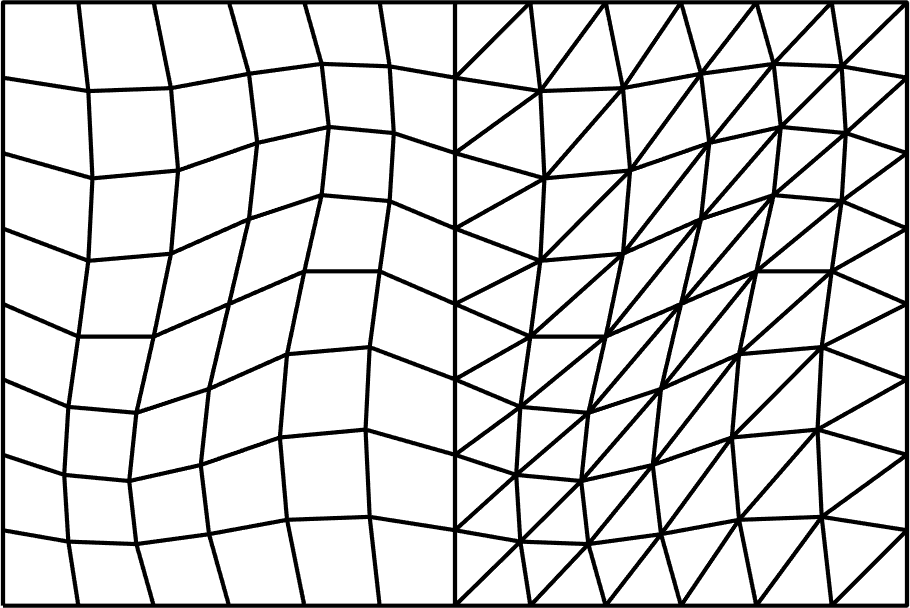
\includegraphics[width=.45\textwidth]{figs/hybrid_mesh.png}
%}}
\caption{Coarsest hybrid mesh used for convergence studies. }
\end{figure}

\begin{figure}
\centering
%\subfloat{\raisebox{2.85em}{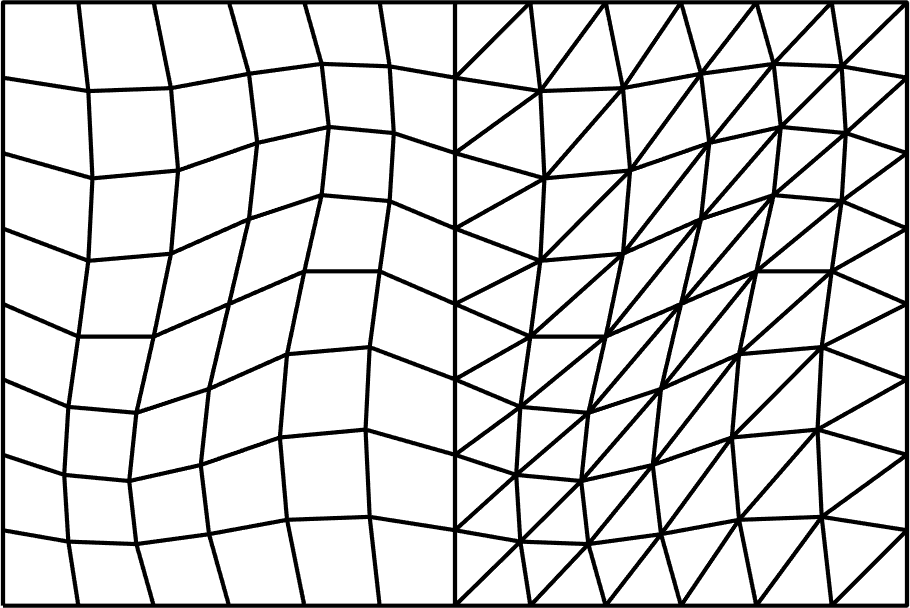
\includegraphics[width=.45\textwidth]{figs/hybrid_mesh.png}}}
%\hspace{.25em}
%\subfloat[Option~\ref{opt:1}]{
\begin{tikzpicture}
\begin{loglogaxis}[
    width=.7\textwidth,
    xlabel={Mesh size $h$},
    ylabel={$L^2$ errors}, 
    xmax=.7,
    ymin=1e-5, ymax=5,
    legend pos=south east, legend cell align=left, legend style={font=\tiny},	
    xmajorgrids=true, ymajorgrids=true, grid style=dashed,
    legend entries={Option~\ref{opt:1},Option~\ref{opt:2},Option~\ref{opt:3}}    
]
\pgfplotsset{
cycle list={{blue, mark=*}, {red, dashed ,mark=triangle*}, {black, mark=square*}}
}
\addplot+[semithick, mark options={solid, fill=markercolor}]
coordinates{(0.333333,2.29471)(0.166667,1.55868)(0.0833333,0.746603)(0.0416667,0.274017)};
\addplot+[semithick, mark options={solid, fill=markercolor}]
coordinates{(0.333333,2.39742)(0.166667,1.63628)(0.0833333,0.885414)(0.0416667,0.435973)};
\addplot+[semithick, mark options={solid, fill=markercolor}]
coordinates{(0.333333,1.74989)(0.166667,0.687578)(0.0833333,0.169682)(0.0416667,0.0350721)};
\addplot+[semithick, mark options={solid, fill=markercolor}]
coordinates{(0.333333,1.06222)(0.166667,0.267115)(0.0833333,0.0395222)(0.0416667,0.00569986)};
\addplot+[semithick, mark options={solid, fill=markercolor}]
coordinates{(0.333333,1.11474)(0.166667,0.265955)(0.0833333,0.0382799)(0.0416667,0.00492061)};
\addplot+[semithick, mark options={solid, fill=markercolor}]
coordinates{(0.333333,0.51272)(0.166667,0.0625001)(0.0833333,0.00835287)(0.0416667,0.00120101)};
\addplot+[semithick, mark options={solid, fill=markercolor}]
coordinates{(0.333333,0.321422)(0.166667,0.037836)(0.0833333,0.00336728)(0.0416667,0.000268691)};
\addplot+[semithick, mark options={solid, fill=markercolor}]
coordinates{(0.333333,0.364547)(0.166667,0.0393928)(0.0833333,0.00357584)(0.0416667,0.000392883)};
\addplot+[semithick, mark options={solid, fill=markercolor}]
coordinates{(0.333333,0.133053)(0.166667,0.0122055)(0.0833333,0.000730739)(0.0416667,4.37208e-05)};
\addplot+[semithick, mark options={solid, fill=markercolor}]
coordinates{(0.333333,0.10556)(0.166667,0.00654941)(0.0833333,0.000267376)(0.0416667,NaN)};
\addplot+[semithick, mark options={solid, fill=markercolor}]
coordinates{(0.333333,0.0955729)(0.166667,0.00649092)(0.0833333,0.000236043)(0.0416667,NaN)};
\addplot+[semithick, mark options={solid, fill=markercolor}]
coordinates{(0.333333,0.0525951)(0.166667,0.00229986)(0.0833333,6.74854e-05)(0.0416667,NaN)};
\node at (axis cs:.45, 2.25) {$N = 1$};
\node at (axis cs:.45,.8) {$N = 2$};
\node at (axis cs:.45,.225) {$N = 3$};
\node at (axis cs:.45,.075) {$N = 4$};
\end{loglogaxis}
\end{tikzpicture}

%}
%\subfloat[Option~\ref{opt:2}]{
%\begin{tikzpicture}
%\begin{loglogaxis}[
%    width=.49\textwidth,
%    xlabel={Mesh size $h$},
%    ylabel={$L^2$ errors}, 
%%    xmax=1,
%    ymin=1e-5, ymax=5,
%    legend pos=south east, legend cell align=left, legend style={font=\tiny},	
%    xmajorgrids=true, ymajorgrids=true, grid style=dashed,
%    legend entries={$N=1$, $N=2$, $N=3$, $N=4$}    
%]
%\pgfplotsset{
%cycle list name=color
%}
%\addplot+[semithick, mark options={solid, fill=markercolor}]
%coordinates{(0.333333,2.39742)(0.166667,1.63628)(0.0833333,0.885414)(0.0416667,0.435973)};
%\addplot+[semithick, mark options={solid, fill=markercolor}]
%coordinates{(0.333333,1.11474)(0.166667,0.265955)(0.0833333,0.0382799)(0.0416667,0.00492061)};
%\addplot+[semithick, mark options={solid, fill=markercolor}]
%coordinates{(0.333333,0.364547)(0.166667,0.0393928)(0.0833333,0.00357584)(0.0416667,0.000392883)};
%\addplot+[semithick, mark options={solid, fill=markercolor}]
%coordinates{(0.333333,0.0955729)(0.166667,0.00649092)(0.0833333,0.000236043)(0.0416667,NaN)};
%\end{loglogaxis}
%\end{tikzpicture}
%}
%
%\subfloat[Option~\ref{opt:3}]{
%\begin{tikzpicture}
%\begin{loglogaxis}[
%    width=.49\textwidth,
%    xlabel={Mesh size $h$},
%    ylabel={$L^2$ errors}, 
%%    xmax=1,
%    ymin=1e-5, ymax=5,
%    legend pos=south east, legend cell align=left, legend style={font=\tiny},	
%    xmajorgrids=true, ymajorgrids=true, grid style=dashed,
%    legend entries={$N=1$, $N=2$, $N=3$, $N=4$}    
%]
%\pgfplotsset{
%cycle list name=color
%}
%\addplot+[semithick, mark options={solid, fill=markercolor}]
%coordinates{(0.333333,1.74989)(0.166667,0.687578)(0.0833333,0.169682)(0.0416667,0.0350721)};
%\addplot+[semithick, mark options={solid, fill=markercolor}]
%coordinates{(0.333333,0.51272)(0.166667,0.0625001)(0.0833333,0.00835287)(0.0416667,0.00120101)};
%\addplot+[semithick, mark options={solid, fill=markercolor}]
%coordinates{(0.333333,0.133053)(0.166667,0.0122055)(0.0833333,0.000730739)(0.0416667,4.37208e-05)};
%\addplot+[semithick, mark options={solid, fill=markercolor}]
%coordinates{(0.333333,0.0525951)(0.166667,0.00229986)(0.0833333,6.74854e-05)(0.0416667,NaN)};
%\end{loglogaxis}
%\end{tikzpicture}
%}
\caption{Convergence of $L^2$ errors for the isentropic vortex solution for Option~\ref{opt:1}, Option~\ref{opt:2}, and Option~\ref{opt:3} for $N = 1,\ldots, 4$.}
\end{figure}

\begin{itemize}
\item \note{GQ-GQ hexes, tris}
\item \note{GLL-GQ hexes, tris}
\item \note{GQ-GLL hexes, GLL tris}
\end{itemize}

\section{Conclusions}

\note{GLL quadrature really is super convenient.}

\note{Need mortar to .}


%\section{Acknowledgments} The author thanks David C.\ Del Rey Fernandez for 

%\appendix
%
%\section{A modified Geometric terms}


\bibliographystyle{unsrt}
\bibliography{dg}



\end{document}


